%%%%%%%%%%%%%%%%%%%%%%%%%%%%%%%%%%%%%%%%%
% Masters/Doctoral Thesis 
% LaTeX Template
%
% This template was downloaded from:
% http://www.LaTeXTemplates.com
%
% Version 2.x major modifications by:
% Vel (vel@latextemplates.com)
%
% This template is based on a template by:
% Steve Gunn (http://users.ecs.soton.ac.uk/srg/softwaretools/document/templates/)
% Sunil Patel (http://www.sunilpatel.co.uk/thesis-template/)
%
% Template license:
% CC BY-NC-SA 3.0 (http://creativecommons.org/licenses/by-nc-sa/3.0/)
%
%%%%%%%%%%%%%%%%%%%%%%%%%%%%%%%%%%%%%%%%%

%----------------------------------------------------------------------------------------
%	PACKAGES AND OTHER DOCUMENT CONFIGURATIONS
%----------------------------------------------------------------------------------------
\documentclass[
11pt, % The default document font size, options: 10pt, 11pt, 12pt
%oneside, % Two side (alternating margins) for binding by default, uncomment to switch to one side
english, % ngerman for German
singlespacing, % Single line spacing, alternatives: onehalfspacing or doublespacing
%draft, % Uncomment to enable draft mode (no pictures, no links, overfull hboxes indicated)
%nolistspacing, % If the document is onehalfspacing or doublespacing, uncomment this to set spacing in lists to single
%liststotoc, % Uncomment to add the list of figures/tables/etc to the table of contents
%toctotoc, % Uncomment to add the main table of contents to the table of contents
%parskip, % Uncomment to add space between paragraphs
%nohyperref, % Uncomment to not load the hyperref package
headsepline, % Uncomment to get a line under the header
%chapterinoneline, % Uncomment to place the chapter title next to the number on one line
%consistentlayout, % Uncomment to change the layout of the declaration, abstract and acknowledgements pages to match the default layout
]{MastersDoctoralThesis} % The class file specifying the document structure
%%%%%
\usepackage[Lenny]{fncychap}
\ChNameUpperCase
\ChNumVar{\fontsize{40}{42}\usefont{OT1}{ptm}{m}{n}\selectfont}
\ChTitleVar{\Large\bfseries}
%%%%%
\usepackage{ragged2e}
\justifying
\usepackage{physics}
\usepackage{float}
\usepackage{braket}
\usepackage{amsmath}\setcounter{MaxMatrixCols}{20}
\usepackage{amsthm} % Provides the environments of proofs
\renewcommand\qedsymbol{QED}
\usepackage[short]{optidef}
\usepackage{amsfonts,amssymb}
\usepackage[utf8]{inputenc} % Required for inputting international characters
\usepackage[T1]{fontenc} % Output font encoding for international characters
\usepackage{mathpazo} % Use the Palatino font by default
\usepackage{minted}
\usepackage[sorting=none, style=ieee]{biblatex}
\usepackage{wrapfig}
% THEOREMS AND DEFINITIONS
\usepackage{tcolorbox}

\tcbuselibrary{breakable,theorems,skins}
%-----------------------------------------------
% Theorem environments definitions
\newcounter{theo} % Extern counter for theorems
\newtcbtheorem[auto counter, number within = chapter]% init options
{theorem}% name environment
{Theorem}% Title
{enhanced,before title={\stepcounter{theo}},colback=blue!10,colframe=blue!35!black,fonttitle=\bfseries,%
attach boxed title to top left={xshift=5mm,yshift*=-\tcboxedtitleheight/2},%
boxed title style={colback=blue!35!black}}% options
{th}% label prefix

\newtcbtheorem[auto counter, number within = chapter]% init options
{corollary}% name environment
{Corollary}% Title
{enhanced,colback=green!10,colframe=green,fonttitle=\bfseries,colbacktitle=green!10,coltitle=black,%
attach boxed title to top left={xshift=5mm,yshift*=-\tcboxedtitleheight/2},%
boxed title style={boxrule=0.6pt}}% options
{co}% label prefix

\newtcbtheorem[auto counter, number within = chapter]% init options
{definition}% name environment
{Definition}% Title
{enhanced,colback=yellow!10,colframe=yellow,fonttitle=\bfseries,colbacktitle=yellow!10,coltitle=black,%
attach boxed title to top left={xshift=5mm,yshift*=-\tcboxedtitleheight/2},%
boxed title style={boxrule=0.6pt}}% options
{def}% label prefix

%------------------------------------------------


\addbibresource{references.bib} % The filename of the bibliography
\usepackage[autostyle=true]{csquotes} % Required to generate language-dependent quotes in the bibliography
\usepackage{hyperref}
\usepackage{orcidlink}
%----------------------------------------------------------------------------------------
%	MARGIN SETTINGS
%----------------------------------------------------------------------------------------

\geometry{
	paper=a4paper, % Change to letterpaper for US letter
	inner=2.0cm, % Inner margin 2.5
	outer=2.5cm, % Outer margin 3.8
	bindingoffset=.5cm, % Binding offset
	top=1.5cm, % Top margin
	bottom=1.5cm, % Bottom margin
	%showframe, % Uncomment to show how the type block is set on the page
}

%----------------------------------------------------------------------------------------
%	THESIS INFORMATION
%----------------------------------------------------------------------------------------

\thesistitle{Transmission Expansion Planning by Quantum Annealing} % Your thesis title, this is used in the title and abstract, print it elsewhere with \ttitle
\supervisor{Dr. Álvaro Díaz Fernández \orcidlink{0000-0001-9432-7845}\\
Dr. Oriol Raventós Morera \orcidlink{0000-0002-0512-4331}} % Your supervisor's name, this is used in the title page, print it elsewhere with \supname
\examiner{} % Your examiner's name, this is not currently used anywhere in the template, print it elsewhere with \examname
\degree{MSc in Quantum Computing} % Your degree name, this is used in the title page and abstract, print it elsewhere with \degreename
\author{Sergio López Baños \orcidlink{0009-0001-4873-7437}} % Your name, this is used in the title page and abstract, print it elsewhere with \authorname
\addresses{} % Your address, this is not currently used anywhere in the template, print it elsewhere with \addressname

\subject{Quantum Computing} % Your subject area, this is not currently used anywhere in the template, print it elsewhere with \subjectname
\keywords{} % Keywords for your thesis, this is not currently used anywhere in the template, print it elsewhere with \keywordnames
\university{\href{https://www.nebrija.com}{Nebrija University}} % Your university's name and URL, this is used in the title page and abstract, print it elsewhere with \univname
\department{\href{https://www.dlr.de/}{DLR - Deutsches Zentrum
für Luft- und Raumfahrt}} % Your department's name and URL, this is used in the title page and abstract, print it elsewhere with \deptname
\group{\href{https://www.dlr.de/ve/en/desktopdefault.aspx/tabid-12472/21440_read-49440/}{Institute of Networked Energy Systems}} % Your research group's name and URL, this is used in the title page, print it elsewhere with \groupname
\faculty{\href{https://www.dlr.de/}{Research Center}} % Your faculty's name and URL, this is used in the title page and abstract, print it elsewhere with \facname

\AtBeginDocument{
\hypersetup{pdftitle=\ttitle} % Set the PDF's title to your title
\hypersetup{pdfauthor=\authorname} % Set the PDF's author to your name
\hypersetup{pdfkeywords=\keywordnames} % Set the PDF's keywords to your keywords
}

\begin{document}

\frontmatter % Use roman page numbering style (i, ii, iii, iv...) for the pre-content pages
\pagestyle{plain} % Default to the plain heading style until the thesis style is called for the body content

%----------------------------------------------------------------------------------------
%	TITLE PAGE
%----------------------------------------------------------------------------------------

\begin{titlepage}
\pagecolor{RojoNebrija}
\color{white}
\begin{center}


\centerline{\includegraphics[width=220mm]{logos/LogoPortada.png}}
%{\scshape\LARGE \univname\par}\vspace{1.5cm} % University name
%\textsc{\Large Master Thesis}\\[0.5cm] % Thesis type

\HRule \\[0.4cm] % Horizontal line
{\huge \bfseries \ttitle\par}\vspace{0.4cm} % Thesis title
\HRule \\[1.5cm] % Horizontal line
 
\begin{minipage}[t]{0.4\textwidth}
\begin{flushleft} \large
\emph{\textbf{Author:}}\\
\item {\authorname} % Author name - remove the \href bracket to remove the link
\end{flushleft}
\end{minipage}
\begin{minipage}[t]{0.4\textwidth}
\begin{flushright} \large
\emph{\textbf{Supervisors:}} \\
{\supname} % Supervisor name - remove the \href bracket to remove the link  
\end{flushright}
\end{minipage}\\[3cm]
 
\vfill

\large \textit{A thesis submitted in fulfilment of the requirements \\ for the degree of \degreename \\ in Nebrija University.}\\[0.3cm] % University requirement text
\textit{The thesis was carried out in}\\[0.4cm]
\changeurlcolor{white}\groupname\\\deptname\\[1cm] % Research group name and department name
\vfill
\centerline{{\colorbox{white}{\makebox(608,75){\includegraphics[scale=0.65]{logos/DLR_Logo_EN_schwarz.png}}}}}
 % University/department logo - uncomment to place it

%{\large \today}\\[4cm] % Date 
\vfill
\end{center}
\end{titlepage}
\pagecolor{white}
%----------------------------------------------------------------------------------------
%	DECLARATION PAGE
%----------------------------------------------------------------------------------------

\begin{declaration}
\addchaptertocentry{\authorshipname} % Add the declaration to the table of contents
\noindent I, \authorname, declare that this thesis titled, \enquote{\ttitle} and the work presented in it are my own. I %confirm that:

\begin{itemize} 
\item This work was done wholly or mainly while in candidature for a research degree at this University.
\item Where any part of this thesis has previously been submitted for a degree or any other qualification at this University or any other institution, this has been clearly stated.
\item Where I have consulted the published work of others, this is always clearly attributed.
\item Where I have quoted from the work of others, the source is always given. With the exception of such quotations, this thesis is entirely my own work.
\item I have acknowledged all main sources of help.
\item Where the thesis is based on work done by myself jointly with others, I have made clear exactly what was done by others and what I have contributed myself.
\end{itemize}
\vspace{5mm}
 \begin{center}
   \noindent \textbf{Signed:} \color{blue}Sergio López Baños\color{black}.\\
\rule[0.5em]{25em}{0.5pt}\\ % This prints a line for the signature
\noindent \textbf{Date:} \color{blue} June 12, 2023\color{black}.\\
\rule[0.5em]{25em}{0.5pt} % This prints a line to write the date  
 \end{center}
\end{declaration}

\cleardoublepage

%----------------------------------------------------------------------------------------
%	QUOTATION PAGE
%----------------------------------------------------------------------------------------

%\vspace*{0.2\textheight}

%\noindent\enquote{\itshape Thanks to my solid academic training, today I can write hundreds of words on virtually any topic without possessing a shred of information, which is how I got a good job in journalism.}\bigbreak

%\hfill Dave Barry

%----------------------------------------------------------------------------------------
%	ABSTRACT PAGE
%----------------------------------------------------------------------------------------

\begin{abstract}
\addchaptertocentry{\abstractname} % Add the abstract to the table of contents
The \textit{transmission expansion planning} problem (TEP) is a \textit{mixed-integer linear programming} (MILP) problem that aims at finding the optimal way to expand the capacity of an energy system. It decides how many components to build in order to satisfy the energy demand on a distributed energy system with a high share of renewable energy sources. The TEP scales badly using classical algorithms and, at the same time, energy system models are getting larger and more complex due to the integration of decentralized weather-dependent renewable energy sources, sector coupling and the increase of storage components. Currently, the problem is often linearized or the scope and granularity of the model are reduced using clustering algorithms. For this reason, any computational time reduction will have substantial implications in closing the granularity gap between what the current models can solve and the desired resolution needed by energy system operators.\\
Quantum annealers are single-purpose quantum computers specialized in solving combinatorial optimization problems. Because of the maturity of quantum computers large problems cannot be tackled purely with a quantum computer. Due to this fact, we show how to solve a small TEP problem fully with a quantum annealer and scale the problem until an embedding is not possible with the current hardware. Moreover, we propose a decomposition protocol for the TEP problem so that we can use a hybrid classic-quantum approach to tackle bigger problems by addressing the binary master problem to a quantum annealer and a set of sub-problems to classical solvers. This would allow us to take advantage of cutting-edge classical algorithms to solve the linear part along with quantum annealers to get, hopefully, a speed-up from it.
\end{abstract}

%----------------------------------------------------------------------------------------
%	ACKNOWLEDGEMENTS
%----------------------------------------------------------------------------------------

\begin{acknowledgements}
\addchaptertocentry{\acknowledgementname} % Add the acknowledgements to the table of contents
I have no words to express my gratitude to my supervisor Álvaro Díaz Fernández not only for his lecture notes, corrections and feedback on the thesis but also for his academic advices. His expertise and attention to the details have played a crucial role in the success of my thesis. \\\\
Also, I am grateful for the working environment and the support that the German Aerospace Center (DLR) has offered to me for the preparation of this thesis at the Institute of Networked Energy Systems. In particular, I am deeply thankful to Oriol Raventós Morera, for introducing me to the research world and for their insightful comments and suggestions.\\\\
Lastly, I would like to thanks my family. For their support in every decision I made and for their unconditional love.
\end{acknowledgements}

%----------------------------------------------------------------------------------------
%	LIST OF CONTENTS/FIGURES/TABLES PAGES
%----------------------------------------------------------------------------------------

\tableofcontents % Prints the main table of contents

\listoffigures % Prints the list of figures

\listoftables % Prints the list of tables

\listofalgorithms % Prints the list of algorithms
%----------------------------------------------------------------------------------------
%	ABBREVIATIONS
%----------------------------------------------------------------------------------------

\begin{abbreviations}{ll} % Include a list of abbreviations (a table of two columns)
\textbf{AQC} & \textbf{A}diabatic \textbf{Q}uantum \textbf{C}omputing \\
\textbf{BD} &  \textbf{B}ender \textbf{D}ecomposition\\
\textbf{DDP} & \textbf{D}ual \textbf{D}ynamic \textbf{P}rogramming\\
\textbf{HQC} & \textbf{H}ybrid \textbf{Q}uantum-\textbf{C}lassical\\
\textbf{HPC} & \textbf{H}igh \textbf{P}erformance \textbf{C}omputing\\
\textbf{MP} & \textbf{M}aster \textbf{P}roblem \\
\textbf{NISQ} & \textbf{N}oisy  \textbf{I}ntermediate-\textbf{S}cale  \textbf{Q}uantum\\
\textbf{SA} & \textbf{S}imulated \textbf{A}nnealing \\
\textbf{SP} & \textbf{S}ub-\textbf{P}roblem \\
\textbf{QA} & \textbf{Q}uantum \textbf{A}nnealing \\
\textbf{QPU} & \textbf{Q}uantum \textbf{P}rocessing \textbf{U}nit \\
\textbf{QUBO} & \textbf{Q}uadratic \textbf{U}nconstrained \textbf{B}inary \textbf{O}ptimization\\
\textbf{TEP} & \textbf{T}ransmission \textbf{E}xpansion \textbf{P}lanning\\
\textbf{TSP} & \textbf{T}ravelling \textbf{S}alesman \textbf{P}roblem\\

\end{abbreviations}

%----------------------------------------------------------------------------------------
%	PHYSICAL CONSTANTS/OTHER DEFINITIONS
%----------------------------------------------------------------------------------------

%\begin{constants}{lr@{${}={}$}l} % The list of physical constants is a three column table

% The \SI{}{} command is provided by the siunitx package, see its documentation for instructions on how to use it

%Speed of Light & $c_{0}$ & \SI{2.99792458e8}{\meter\per\second} (exact)\\
%Constant Name & $Symbol$ & $Constant Value$ with units\\

%\end{constants}

%----------------------------------------------------------------------------------------
%	SYMBOLS
%----------------------------------------------------------------------------------------

%\begin{symbols}{lll} % Include a list of Symbols (a three column table)

%$a$ & distance & \si{\meter} \\
%$P$ & power & \si{\watt} (\si{\joule\per\second}) \\
%Symbol & Name & Unit \\

%\addlinespace % Gap to separate the Roman symbols from the Greek

%$\omega$ & angular frequency & \si{\radian} \\

%\end{symbols}

%----------------------------------------------------------------------------------------
%	DEDICATION
%----------------------------------------------------------------------------------------

\dedicatory{Dedico esta Tesis de Máster a mis padres, cuyo esfuerzo ha permitido que estudiase en la universidad y cuyos consejos me han guiado, inspirado y motivado en el camino.} 

%----------------------------------------------------------------------------------------
%	THESIS CONTENT - CHAPTERS
%----------------------------------------------------------------------------------------

\mainmatter % Begin numeric (1,2,3...) page numbering

\pagestyle{thesis} % Return the page headers back to the "thesis" style

% Include the chapters of the thesis as separate files from the Chapters folder
% Uncomment the lines as you write the chapters
% Chapter Template

\chapter{Introduction} % Main chapter title

\label{Chapter1} % Change X to a consecutive number; for referencing this chapter elsewhere, use \ref{ChapterX}

%----------------------------------------------------------------------------------------
%	SECTION 1
%----------------------------------------------------------------------------------------
%
% Statment of the problem + Motivation
%
Quantum computing is a new paradigm of computation whose importance is growing not only because of its promising speed-up over classical computers in some problems, such as combinatorial optimization problems, but also due to the fact that we are building transistors in a scale where quantum effects are starting to become relevant. Combinatorial optimization problems are common among industry albeit more research needs to be done to get insight about how quantum computing could help to solve industry challenges. There is already a large industry research in finance [\textbf{REFERENCIAS}], route planning [\textbf{REFERENCIAS}], cybersecurity [\textbf{REFERENCIAS}] and life sciences, among others. The research on applications of quantum computing to the energy sector has just began in the last years. The goal of this work to contribute to its progress. There are only a few active research projects, like Q-Grid by e-On\,\cite{Fernandez-Campoamor2021CommunityAnnealing} or EnerQuant by Fraunhofer.\\\\
\begin{figure}[H]
  \begin{center}
\includegraphics[width=0.9\textwidth]{Figures/Europe-Grid.png}
  \end{center}
  \caption{Clustered European transmission network model from PyPSA-EUR\,\cite{PyPSA-Eur:PyPSA-Eur}. }
\end{figure}
Energy system models are getting larger and more complex due to the integration of decentralized weather-dependent renewable energy sources, intermittent loads, sector coupling and the increase of storage components. For instance, the renewable energy produced by the integration of solar panels in dwellings is thought to be integrated to the grid if the consumers are not using it, but the grid infrastructure is not evolving accordingly to the new energy paradigm. As a consequence, energy from private sources cannot be added to the grid which implies the efficiency of solar panels has to be decreased or the excess of energy has to be dropped. A good infrastructure would solve these problems by addressing the excess of energy to where it is required and by storing the excess so it can be used later, e.g., to charge an electric car. In this way, the energy would be efficiently distributed and energy companies could offer better prices to their consumers while safeguarding the environment by reducing their carbon footprints. Furthermore, an increment of the quantity of detailed data about energy consumption -- smart meters -- would extend the spatial and temporal resolution, i.e., the grid status of a region, so that better managing and expansion planning decisions can be made in order to satisfy the customer demand efficiently.\\\\ 
The problem we tackle in the present work is called transmission expansion planning (TEP) problem, which is a \textit{mixed integer linear problem} (MILP), with NP complexity, i.e., an increment in the spatial and time resolution entails an exponential growth in the number of variables for the MILP making large problems intractable for a classical computer. Currently, the scope and granularity of the model are reduced using clustering algorithms. For this reason, any computational time reduction will have substantial implications in closing the granularity gap between what the current models can solve and the desired resolution needed by energy system operators.\\\\
Quantum computers are the candidates to solve NP-hard problems such as MILP, by making the complexity of the problem scale polynomically as the systems size grows. Concretely, quantum analog computers are single-purpose quantum computers specialised in solving combinatorial optimization problems. The size of analog computers, i.e., the number of qubits of the system is greater than the general purpose quantum computers -- digital computers -- such as the ones from IBM that are based in the successive applications of quantum gates, e.g., Osprey with 433 qubits.
%
% Objectives of my thesis
%
Although quantum computers are getting bigger every few years they are not mature enough for solving many real-world problems where the number of variables scale exponentially. Also, we have to take into account that quantum computers are hugely affected by the environmental conditions -- Noisy Intermediate-Scale Quantum (NISQ) era --, so there are errors during a code execution and the execution time has to be short enough so that it does not exceed quantum decoherence. The current maturity of quantum computers requires of a hybrid quantum-classical approach to tackle real-world problems. The hybrid approach combines classical solvers and cutting-edge classical algorithms with quantum solvers that add the speed-up where it is possible.\\\\
A benchmark of how a TEP problem can be scaled until a quantum solver is not able to find a solution is provided among with a scheme to decompose a large TEP problem into a small enough master problem that can be addressed by a quantum computer and a sub-problem addressed by a classical computer. \\\\
% Structure of the thesis
%
The present work is structured as follows. Chapter\,\ref{Chapter2} guides through the foundations of adiabatic quantum computing. Chapter\,\ref{Chapter3} describes Benders' decomposition techniques. Chapter\,\ref{Chapter4} solves a transmission expansion problem by starting with a small network solved by a pure quantum annealer and ending up with a bigger network that requires from hybrid solvers. Conclusions and outlook are drawn in Chapter\,\ref{Chapter5}.

% Chapter 2

\chapter{Adiabatic quantum computing} % Main chapter title

\label{Chapter2} % For referencing the chapter elsewhere, use \ref{Chapter1} 
In the present chapter we show a paradigm of quantum computation known as \textit{adiabatic quantum computing} (AQC), see Ref. \cite{Farhi2000QuantumEvolution}. We start by sketching the rough idea of the adiabatic theorem to finally derive a formal proof of it. We also expose one application of AQC to solve \textit{quadratic unconstrained binary optimization} (QUBO) problems, known as \textit{quantum annealing} (QA), see Ref. \cite{Kadowaki1998QuantumModel}.

%%%%%%%%%%%%%%%%%%%%%%%%%%%%%%%%%%%%%%%%%%%%%%%%%%%%%%%%%%%%%%%%%%%%%%%%%%%%%%%%%%%%%%%%%%%%%%%%%%%%%%%%%%
%     1.1 ADIABATIC APPROXIMATION
%%%%%%%%%%%%%%%%%%%%%%%%%%%%%%%%%%%%%%%%%%%%%%%%%%%%%%%%%%%%%%%%%%%%%%%%%%%%%%%%%%%%%%%%%%%%%%%%%%%%%%%%%%
\section{The adiabatic theorem}
Quoting Sarandy and Lidar\,\cite{Sarandy2005AdiabaticSystems},
\begin{displayquote}
\textit{The theorem posits, roughly, that if a state is an instantaneous eigenstate of a sufficiently slowly varying Hamiltonian at one time, then it will remain an eigenstate at later times, while its eigenenergy evolves continuously.}
\end{displayquote}
\subsection{The adiabatic protocol}
We need to construct an initial Hamiltonian $\mathcal{H}(t=0) = \mathcal{H}_{i}$ whose ground state is known and whose time evolution, $t \in \left[0,T\right]$ -- where $T$ is the total evolution time -- leads to a Hamiltonian $\mathcal{H}(t=T) = \mathcal{H}_{f}$ that encodes the solution to our problem. Mathematically we can write a linear schedule between the initial and target Hamiltonian,
\begin{equation}
\label{eq:Htime}
    \mathcal{H}(t) = \left(1-\frac{t}{T}\right)\mathcal{H}_{i} + \left(\frac{t}{T} \right)\mathcal{H}_{f}
\end{equation}
The adiabatic theorem guarantees that if we start with an initial Hamiltonian $\mathcal{H}_{i}$ in a given eigenspace and the evolution is carried out sufficiently slowly -- in further sections we demonstrate what slowly means in detail -- then we end up in the equivalent eigenspace of the final Hamiltonian $\mathcal{H}_{f}$. \\\\
To summarise:
\begin{itemize}
    \item \textbf{Step 1 (Mapping):} Map the problem into a Hamiltonian $\mathcal{H}_{f}$ eigenstate. Typically, the problem is encoded in the ground state.
    \item \textbf{Step 2 (Initialise $\mathcal{H}_{i}$):} Initialise the system in the ground state of a Hamiltonian $\mathcal{H}_{i}$, easy to compute and to prepare. We need to pick a Hamiltonian whose ground state is easy to compute, e.g., the ground state of $\mathcal{H} = - \sum_{i}^{n}\hat{\sigma}_{i}^{x}$ is the eigenvector $\ket{+}^{\otimes n}$.
    \item \textbf{Step 3 (Adiabatic Theorem):} Slowly evolve the system from $H_{i}$ to $H_{f}$. The adiabatic theorem guarantees that, under certain conditions that will be explained later, the system will end up in the ground state of $H_{f}$.
    \item \textbf{Step 4 (Measure):} Measure the eigenstate of $H_{f}$. The result provides a ground eigenvector that encodes a solution to our problem.
\end{itemize}
Notice that we wrote in \textbf{Step 4 (Measure)} that the result of the measurement provides "a solution" not "the solution". This is because there are two possibilities for a finite-dimensional Hamiltonian:
\begin{itemize}
    \item \textbf{Non-degenerate Hamiltonian:} We start with an initial Hamiltonian $\mathcal{H}_{i}$ in its ground eigenstate $\ket{g(t=0)}$ and end up in the equivalent eigenstate -- ground state -- of the final Hamiltonian $\mathcal{H}_{f}$ where the eigenvalue is $E_{g}(t=T)$ and the eigenvector is $\ket{g(t=T)}$.
    \item \textbf{Degenerate Hamiltonian:} We start with an initial Hamiltonian $\mathcal{H}_{i}$ in its ground eigenspace spanned by $\{\ket{g^{i}(t=0)}\}_{i \in \left[1,d\right]}$, where $d$ is the degeneracy of the ground state, and end up in the equivalent eigenspace of the final Hamiltonian $\mathcal{H}_{f}$ with eigenvalue $E_{g}(t=T)$.
\end{itemize}
Intuitively, one can think that a problem can have multiple configurations that leads to the same minimum eigenvalue.
%%%%%%%%%%%%%%%%%%%%%%%%%%%%%%%%%%%%%%%%%%%%%%%%%%%%%%%%%%%%%%
\subsection{The adiabatic theorem: a first approach}
We now provide a simple argument to build intuition into the adiabatic theorem. The next section will be devoted to a formal proof. In order to continue, let us define the following dimensionless variable
\begin{equation}
    s \equiv \frac{t}{T} \ , \quad s \in [0,1]
\end{equation}
Then, the state of an $n$-qubit system, whose instantaneous spectrum is discrete and non-degenerate, can be written as a linear combination of the instantaneous eigenstates of the Hamiltonian $\ket{\psi(s)} = \sum_{i}c_{i}(s)\ket{i(s)}$ as function of $s$. Its evolution is given by the time-dependent Schrödinger equation, see Appx.\,\ref{AppendixA},
\begin{equation}
\label{eq:GeneralEv}
    i\hbar \ket{\dot{\psi}(s)} = \mathcal{H}(s) \ket{\psi(s)}
\end{equation}
In general, Eq.\,\eqref{eq:GeneralEv} represents a system of coupled differential equations for the evolution of the state $\ket{\psi(s)}$ which has a non-trivial solution. However, we can re-write the Hamiltonian in diagonal form using the change-of-basis matrix $U(s)$,
\begin{equation}
    \mathcal{H}_{d}(s) = U^{-1}(s)\mathcal{H}(s)U(s) = \begin{bmatrix}
           \lambda_{0} & 0 & \hdots & 0 \\
           0 &  \ddots & & \vdots \\
           \vdots &   & \ddots & 0 \\
           0 & \hdots & 0 & \lambda_{2^{n-1}}
         \end{bmatrix}
\end{equation}
We also define $\ket{\psi_{d}(s)} = U^{-1}(s)\ket{\psi(s)}$ as the state we get after applying the inverse transformation $U^{-1}(s)$ to the state $\ket{\psi(s)}$. Using the identity $\mathbb{I} = U(s)U^{-1}(s)$ and multiplying both sides of Eq.\,\eqref{eq:GeneralEv} by $U^{-1}(s)$ yields to
\begin{equation}
     i\hbar U^{-1}(s) \frac{\partial \left(U(s)U^{-1}(s)\ket{\psi(s)}\right)}{\partial s} = U^{-1}(s)\mathcal{H}(s) \left(U(s)U^{-1}(s)\right)\ket{\psi(s)}
\end{equation}
Rearranging terms
\begin{equation}
     i\hbar U^{-1}(s) \frac{\partial U(s)}{\partial s}\ket{\psi_{d}(s)} + i\hbar  \frac{\partial \ket{\psi_{d}(s)}}{\partial s}= \mathcal{H}_{d}(s)\ket{\psi_{d}(s)}
\end{equation}
%Rev
If we assume $\mathcal{H}(s)$ varies slowly, then it is reasonable that $U(s)$ varies slowly as well, $\dot{U}(s) \simeq 0$, which implies
\begin{equation}
    i\hbar  \frac{\partial \ket{\psi_{d}(s)}}{\partial s} \simeq \mathcal{H}_{d}(s)\ket{\psi_{d}(s)}
\end{equation}
Now, the evolution of the state $\ket{\psi_{d}(s)}$ is led by a diagonal Hamiltonian $\mathcal{H}_{d}(s)$ so we have a set of uncoupled differential equations for each amplitude component of the state $\ket{\psi_{d}(s)}$. Furthermore, if the state of the system $\ket{\psi_{d}(s)}$ is an eigenstate of the Hamiltonian $\ket{n(s)}$, then the evolution of our system is conducted inside the eigenspace generated by $\ket{n(s)}$.\\\\
To sum up, under a general evolution such as Eq.\,\eqref{eq:GeneralEv} we get -- in general -- a system of coupled differential equations, but if the adiabatic approximation is satisfied, this evolution is led by a diagonal Hamiltonian, i.e., we get a system of uncoupled differential equations.
\begin{figure}[H]
    \centering
\includegraphics[width=\textwidth]{Figures/Eigenenergies.pdf}
    \caption{An example considering Hamiltonian's eigenenergies as function of dimensionless time $s=t/T$ assuming a problem ecoded in the ground state. \textbf{Left}: When adiabatic conditions are fulfilled, i.e., if the evolution is carried out sufficiently slowly, then our system evolves continuously in time along the ground state. \textbf{Right}: When the evolution is carried out not fulfilling the adiabatic conditions, it could happen that we end up in a different eigenstate if our system absorbs enough energy to jump to next level over the minimum gap $\Delta$. After the evolution we would end up in a different eigenstate of the target Hamiltonian which does not encodes the optimal solution.}
    \label{fig:Eigenenergies}
\end{figure}
Graphically, this means the eigenenergies $E_{n}(s)$ of the Hamiltonian's instantaneous eigenstates $\ket{n(s)}$ do not cross.
Quoting Goldstone \textit{et. al}\,\cite{Farhi2000QuantumEvolution},
\begin{displayquote}
\textit{...if the gap between the two lowest levels, $E_{1} - E_{0}$, is strictly greater than zero for all $0 \leq t \leq T$, then}
\end{displayquote}
\begin{equation}
    \lim_{T\longrightarrow \infty} | \braket{0(t=T) | \psi(t=T)}| = 1
\end{equation}
Equivalently, the probability of being at the ground state of the target Hamiltonian $\mathcal{H}_{f}$ at the end of evolution is 1 if and only if the total time required for the evolution is infinite. Otherwise, the probability of being at the ground state is
\begin{equation}
    || \braket{0(t=T) | \psi(t=T)}||^{2} = 1 - \epsilon^{2}
\end{equation}
where $\epsilon$ takes into account the error due to the adiabatic approximation, $\dot{U}(s) \simeq 0$.
%%%%%%%%%%%%%%%%%%%%%%%%%%%%%%%%%%%%%%%%%%%%%%%%%%%%%%%%%%%%%%%%%%%%%%%%%%%%%%%%%%%%%%%%%%%%%%%%%%%%%%%%%%
%     1.2 ADIABATIC THEOREM
%%%%%%%%%%%%%%%%%%%%%%%%%%%%%%%%%%%%%%%%%%%%%%%%%%%%%%%%%%%%%%%%%%%%%%%%%%%%%%%%%%%%%%%%%%%%%%%%%%%%%%%%%%
\subsection{The adiabatic theorem: a formal derivation}
We start by writing down the Schrödinger equation
\begin{equation}
    i\hbar \frac{\partial \ket{\psi(t)}}{\partial t} = \mathcal{H}(t)\ket{\psi(t)}
\end{equation}
We assume that the instantaneous spectrum of $\mathcal{H}(t)$ is discrete and non-degenerate
\begin{equation}
\label{eq:Hamiltonian}
    \mathcal{H}(t) \ket{n(t)} = E_{n}(t)\ket{n(t)}
\end{equation}
where $\ket{n(t)}$ are the instantaneous eigenstates of the Hamiltonian and $E_{n}(t)$ are the eigenenergies labelled by $n$. Notice that we can label the eigenenergies with a single index because the spectrum is discrete and non-degenerate. For a discrete but degenerate spectrum, we would need an extra index to take into account the degeneracy of each state.\\\\
The eigenstates of the Hamiltonian form an orthonormal basis, so we can expand a given state in that basis
\begin{equation}
\label{eq: EigenvectorExpansion}
    \ket{\psi(t)} = \sum_{n}c_{n}(t)e^{i\theta_{n}(t)} \ket{n(t)}
\end{equation}
where
\begin{equation}
    \theta_{n}(t) = -\frac{1}{\hbar}\int_{0}^{t}E_{n}(t^{\prime})dt^{\prime}
\end{equation}
is the dynamic phase.\\
Substituting Eq.\,\eqref{eq: EigenvectorExpansion} into the Schrödinger equation yields to
\begin{equation}
    \sum_{n}\left[\dot{c}_{n}(t)\ket{n(t)} + c_{n}(t)\ket{\dot{n}(t)}\right]e^{i\theta_{n}(t)} = 0
\end{equation}
Multiplying by $\bra{m(t)}$
\begin{equation}
\label{eq:Coefficients}
    \dot{c}_{m}(t) = - \sum_{n}c_{n}\braket{m(t)|\dot{n}(t)}e^{i\left(\theta_{n}(t) - \theta_{m}(t)\right)}
\end{equation}
We need to re-write $\braket{m(t)|\dot{n}(t)}$ in terms of the Hamiltonian's derivative using Eq.\,\eqref{eq:Hamiltonian}. If we derive that expression with respect to time, we find
\begin{equation}
    \frac{\partial \mathcal{H}(t)}{\partial t}\ket{n(t)} + \mathcal{H}(t)\frac{\partial \ket{n(t)}}{\partial t} = \frac{\partial E_{n}(t)}{\partial t} \ket{n(t)} + E_{n}(t)\frac{\partial \ket{n(t)}}{\partial t} 
\end{equation}
Multiplying the last expression by $\bra{m(t)}$ 
\begin{equation}
    \braket{m(t)|\frac{\partial\mathcal{H}(t)}{\partial t}\ket{n(t)}} + E_{m}(t)\braket{m(t)|\dot{n}(t)} = E_{n}(t)\braket{m(t)|\dot{n}(t)}
\end{equation}
Finally,
\begin{equation}
    \braket{m(t)|\dot{n}(t)} = \frac{1}{E_{n}(t)-E_{m}(t)}\braket{m(t)|\frac{\partial \mathcal{H}(t)}{\partial t}n(t)}
\end{equation}
Substituting into Eq.\,\eqref{eq:Coefficients} and defining $g_{nm}(t)\equiv E_{n}(t) - E_{m}(t)$ as the energy difference as a function of time $t$ between the eigenstates $\ket{m(t)}$ and $\ket{n(t)}$ leads to
\begin{equation}
\label{eq:GeneralCoefficientsNoadiabaticApprox}
    \dot{c}_{m}(t) = -c_{m}(t) \braket{m(t)|\dot{m}(t)} - \sum_{n\neq m} c_{n}(t)\frac{\braket{m(t)|\dot{\mathcal{H}(t)}|n(t)}}{g_{nm}(t)}e^{i\left(\theta_{n}(t) - \theta_{m}(t)\right)}
\end{equation}
Adiabatic evolution is ensured if the coefficients $c_{n}(t)$ evolve independently from each other, i.e., if their dynamical equations do not couple. Mathematically,
\begin{equation}
    \max_{0 \leq t \leq T} \abs{\frac{\braket{m(t)|\dot{\mathcal{H}}(t)|n(t)}}{g_{nm}(t)}} \ll \min_{0\leq t \leq T} \abs{g_{nm}(t)}
\end{equation}
where $T$ is the total evolution time.\\ 
Under the adiabatic approximation the coupling term tends to zero, that is,
\begin{equation}
    \sum_{n\neq m} c_{n}\frac{\braket{m(t)|\dot{\mathcal{H}(t)}|n(t)}}{g_{nm}(t)}e^{i\left(\theta_{n}(t) - \theta_{m}(t)\right)} \to 0
\end{equation}
Therefore, equation Eq.\,\eqref{eq:GeneralCoefficientsNoadiabaticApprox} turns into
\begin{equation}
    \dot{c}_{m}(t) = -c_{m}(t)\braket{m(t)|\dot{m}(t)}
\end{equation}
whose solution is
\begin{equation}
    c_{m}(t) = c_{m}(0)e^{i\gamma_{m}(t)}
\end{equation}
where
\begin{equation}
    \gamma_{m}(t) = i\int_{0}^{t}\braket{m(t^{\prime})|\dot{m}(t^{\prime})}dt^{\prime} \quad \gamma_{m}\in \mathbb{R}
\end{equation}
is the Berry's phase.\\
As we can see, if the system starts in the $m$-th eigenstate of the Hamiltonian, then it will end in the $m$-th eigenstate up to a phase.
%%%%%%%%%%%%%%%%%%%%%%%%%%%%%%%%%%%%%%%%%%%%%%%%%%%%%%%%%%%%%%%%%%%%%%%%
%       TOTAL EVOLUTION TIME
%%%%%%%%%%%%%%%%%%%%%%%%%%%%%%%%%%%%%%%%%%%%%%%%%%%%%%%%%%%%%%%%%%%%%%%%
\subsection{Total evolution time $T$}
In previous sections we stated that under a sufficiently slowly Hamiltonian evolution the adiabatic theorem is satisfied. In this section we define what "slowly" means by deriving an expression to estimate the total time $T$ required for the adiabatic evolution. We also demonstrate that the total time not only depends on the energy gap between the ground state and the first excited state but also on the term $\braket{m(s)|d\mathcal{H}(s)/ds|n(s)}$.\\\\
We start by re-writing Eq.\,\eqref{eq:GeneralCoefficientsNoadiabaticApprox} in terms of the normalised time $s = \frac{t}{T}$ and the Berry's phase.
\begin{equation}
    e^{i\gamma_{m}(sT)}\frac{1}{T}\frac{\partial }{\partial s}\left[c_{m}(sT)e^{-i\gamma_{m}(sT)}\right] = -\sum_{n\neq m} c_{n}(sT) \frac{\braket{m(sT)|\dot{\mathcal{H}}(sT)|n(sT)}}{g_{nm}(sT)}e^{-i\left(\theta_{n}(sT) - \theta_{m}(sT)\right)}
\end{equation}
Notice we have added two Berry's phases terms with opposite sign so they cancel out. Integrating the last equation and rearranging terms leads to
\begin{equation}
\label{eq:Coeff}
    c_{m}(s)e^{-i\gamma_{m}(s)} = c_{m}(0) - \sum_{n\neq m}\int_{0}^{s} ds^{\prime}\frac{F_{nm}(s^{\prime})}{g_{nm}(s^{\prime})}e^{-iT\int_{0}^{s^{\prime}}ds^{\prime\prime}\left(g_{nm}(s^{\prime\prime})\right)}
\end{equation}
This equation express the coefficient $c_{n}(s)$ in term of its initial value $c(0)$ and a summation term that keep the rest of coefficients $c_{m}(s)$ with $m\neq n$, where
\begin{equation}
\label{eq:Fnm}
    F_{nm}(s) = c_{n}(s)\braket{m(s)|\dot{\mathcal{H}}(s)|n(s)} e^{-i\gamma_{m}(s)}
\end{equation}
We can express the integrand of Eq.\,\eqref{eq:Coeff} as a difference between two terms,
\begin{align}
\frac{F_{nm}(s^{\prime})}{g_{nm}(s^{\prime})} e^{-iT\int_{0}^{s^{\prime}}\left(ds^{\prime \prime}g_{nm}(s^{\prime\prime}) \right)}= \\
\frac{i}{T}\left[\frac{d}{ds^{\prime}}\left(\frac{F_{nm}(s^{\prime})}{g^{2}_{nm}(s^{\prime})}e^{-iT\int_{0}^{s^{\prime}}\left(ds^{\prime \prime}g_{nm}(s^{\prime\prime}) \right)}\right) - e^{-iT\int_{0}^{s^{\prime}}\left(ds^{\prime \prime}g_{nm}(s^{\prime\prime}) \right)} \cdot \frac{d}{ds^{\prime}}\left(\frac{F_{nm}(s^{\prime})}{g_{nm}(s^{\prime})}\right)\right] 
 \end{align}
 Substituting the previous result into Eq.\,\eqref{eq:Coeff} leads to
 \begin{equation}
 \begin{split}
      c_{m}(s)e^{-i\gamma_{m}(s)} & = c_{m}(0) + \frac{i}{T}\Biggr[\frac{F_{nm}(0)}{g^{2}_{nm}(0)} - \frac{F_{nm}(s)}{g^{2}_{nm}(s)}e^{-iT\int_{0}^{s}ds^{\prime}g_{nm}(s^{\prime \prime})} \\
      & + \int_{0}^{s}ds^{\prime} e^{-iT\int_{0}^{s^{\prime}}\left(ds^{\prime \prime}g_{nm}(s^{\prime\prime}) \right)} \cdot \frac{d}{ds^{\prime}}\left(\frac{F_{nm}(s^{\prime})}{g_{nm}(s^{\prime})}\right)\Biggr]
\end{split}
\end{equation}
 Assuming the energy gap does not vanish when $T \rightarrow \infty$ and that $d\{F_{nm}(s^{\prime})/g_{nm}^{2}(s^{\prime})\}/ds^{\prime}$ is integrable for all $s \in [0,1]$. Then, Riemann-Lebesgue lemma [\textbf{REFERENCE Tiene sentido ponerla? es un libro}] guarantees that last integral vanishes in the limit $T \rightarrow \infty$. So
  \begin{align}
  \label{eq:cm}
     c_{m}(s)e^{-i\gamma_{m}(s)} = c_{m}(0) + \frac{i}{T}\left[\frac{F_{nm}(0)}{g^{2}_{nm}(0)} - \frac{F_{nm}(s)}{g^{2}_{nm}(s)}e^{-iT\int_{0}^{s}ds^{\prime}g_{nm}(s^{\prime \prime})}\right] 
 \end{align}
 Under the adiabatic conditions there are not mixing terms, i.e., the coefficient $c_{n}(s)$ does not depend on the rest of coefficients. Mathematically,
\begin{equation}
    c_{m}(m) = c_{0}(s)e^{i\gamma_{m}(s)}
\end{equation}
Therefore, we can simplify Eq.\,\eqref{eq:Fnm}
\begin{equation}
    F_{nm}(s) = c_{n}(0)\braket{m(s)|\dot{\mathcal{H}}|n(s)} e^{-i\left[\gamma_{m}(s) - \gamma_{n}(s)\right]}
\end{equation}
 With that simplification we can estimate the total time for an adiabatic evolution by imposing a condition that minimises the second term of Eq.\,\eqref{eq:cm}
 \begin{equation}
     T >> \frac{F}{g^{2}}
 \end{equation}
 where
 \begin{align}
     F = \max_{0 \leq s \leq 1} |c_{n}(0)\braket{m(s)|\frac{d\mathcal{H}(s)}{ds}| n(s)}| \\
     g = \min_{0 \leq s \leq 1} |g_{nm}(s)|
 \end{align}
%-------------------------------------------------------------------------------------
% QUANTUM ANNEALING
%---------------------------------------------------------------------------------------
\section{Quantum annealing}
\textit{Quantum annealing} (QA) takes its name from a classical heuristic algorithm named s\textit{imulated annealing} (SA), see Appx.\,\ref{AppendixB}. It is a particularization of AQC where the Hamiltonian is the Ising's Hamiltonian
\begin{equation}
    \mathcal{H}(s) = -\sum_{ij}\mathcal{J}_{ij}\sigma_{i}^{z}\sigma_{j}^{z} - h\sum_{i}\sigma_{i}^{z}
\end{equation}
The Ising's Hamiltonian's goal is to describe the behaviour of ferromagnetic materials by taking into account its spin distribution. Spin information is given by the eigenvalues of Pauli Z-operators $\sigma^{z}$, where the possibles outcomes are $\{-1,1\}$ corresponding to the eigenvectors $\{\ket{\downarrow},\ket{\uparrow}\}$, respectively.\\\\
Notice we are mapping our mathematical problem into a physical problem. Solving a problem in a classical computer demands computational resources of it, however if the problem is mapped into a physical problem, then it is the nature evolving in time according to the laws of physics what solves the problem. So we are not limited to out classical computational resources but to nature.\\\\
We also need an initial Hamiltonian whose ground state is easy to compute and prepare, e.g.,
\begin{equation}
    \mathcal{H}(s) = -\sum_{i}^{n}\sigma_{i}^{x}
\end{equation}
with ground state $\ket{+}^{n}$. This ground state considers all the possible configurations of our systems with a uniform distribution among them.\\\\
The annealing schedule between these Hamiltonians is given by
\begin{equation}
    \mathcal{H}(s) = -\sum_{ij}\mathcal{J}_{ij}\sigma_{i}^{z}\sigma_{j}^{z} - h\sum_{i}\sigma_{i}^{z} - \Gamma(s)\sum_{i}\sigma_{i}^{x}
\end{equation}
where $\Gamma(s)\sum_{i}\sigma_{i}^{x}$ represents the quantum fluctuations -- single-spin flip -- and $\Gamma(s)$ plays the same role as Temperature in SA. The way of controlling the quantum fluctuations depends on the hardware we are using. The hardware implementation and topology of the quantum computer we have used in the present work is discussed in Appx.\,\ref{AppendixC}.\\\\
Initially, at $s \rightarrow 0$, the dominating term is $\Gamma(s)\sum_{i}\sigma_{i}^{x}$ because $\Gamma(s)$ takes a large value, but at later times $s \rightarrow 1$ $\Gamma(s)$ it takes a value close to zero so the dominating Hamiltonian is $\mathcal{H}(s) = -\sum_{ij}\mathcal{J}_{ij}\sigma_{i}^{z} - h\sum_{i}\sigma_{i}^{z}$ which is the Hamiltonian we are interested in, as it contains the solution to our problem encoded at the ground state.\\\\
\begin{definition}[\textit{Quadratic Unconstrained Binary Optimization} (QUBO)]
   A Quadratic Unconstrained Binary Optimization problem can be written as
\begin{equation}
    \min_{\vec{x}}\vec{x}^{T}Q\vec{x}
\end{equation}
where $\vec{x}\in\{0,1\}^{n}$ are the binary variables of the problem, $n$ is the total number of binary variables and $Q$ is an $n\times n$ matrix whose entries encodes our problem.
\end{definition}
Notice that Ising's Hamiltonian use the binary variables $s_{i} = \{-1,1\}$ but QUBO problems are formulated with the binary variables $x_{i} = \{0,1\}$. The map between Ising and QUBO variables is given by
\begin{equation}
    s_{i} = 2x_{i} -1
\end{equation}
so we can easily re-write the Ising Hamiltonian into a QUBO Hamiltonian and vice versa
\begin{equation}
    \mathcal{H} = \sum_{i,j}x_{i}Q_{ij}x_{j}
\end{equation}
%------------------------------------------------------------------
% Two Heirs Problem
%------------------------------------------------------------------
\subsection{Two Heirs problem}
 As an example suppose we are given a 3-binary QUBO problem where each variable $x_{i} \in \{0,1\}$ represents an asset with an associated value $v_{i}$.\\
\begin{table}[h]
\label{tab:Assets}
\centering
\begin{tabular}{ c | c }
  \hline			
  Index & Value  \\
    \hline		
   0 & 1\\
       \hline		
   1 & 3\\
       \hline		
   2 & 1
\end{tabular}
\caption{Two heirs problem for a given three example assets.}
\end{table}
\\
We have to assign the assets to two heirs, Alice and Bob -- represented by $\{0,1\}$ in QUBO formulation and by $\{-1,1\}$ in Ising formulation, respectively -- so that the difference between the values each heir receives is minimum, which represents our cost function
\begin{equation}
    f(x_{0}, x_{1}, x_{2}) = \abs{\text{Alice}(x_{0}, x_{1}, x_{2}) - \text{Bob}(x_{0}, x_{1}, x_{2})} = \left[\sum_{i}\left((1-x_{i})\cdot v_{i} - x_{i}\cdot v_{i}\right)\right]^{2}
\end{equation}
Notice we are not interested in the sign of our cost function. Therefore, to avoid dealing with signs we take the square of the difference so we know we are minimising a positive quantity.\\\\
We expand the square term to arrive at the QUBO formulation, $\vec{x}^{T}Q\vec{x}$. In order to do that We have to take into account that for $x_{i} \in \{0,1\}$ the following relation holds $x_{i}=x_{i}^{2}$. 
\begin{align}
    \left[\sum_{i}\left((1-x_{i})\cdot v_{i} - x_{i}\cdot v_{i}\right)\right]^{2} = \sum_{i=0}^{2}\sum_{j\neq i}x_{i}v_{i}v_{j}x_{j} - x_{i}v_{i}v_{j}x_{i} - x_{j}v_{i}v_{j}x_{j}
\end{align}
So the QUBO matrix of this example is
\begin{equation}
Q= 
    \begin{bmatrix}
           0 & v_{1}v_{2} & v_{1}v_{3}\\
           v_{2}v_{1} & 0 & v_{2}v_{3}\\
           v_{3}v_{1}& v_{3}v_{2} & 0\\
         \end{bmatrix}
\end{equation}
We can add the contribution of mixed indices in the upper triangular part of the matrix
\begin{equation}
Q= 
    \begin{bmatrix}
           0 & 2v_{1}v_{2} & 2v_{1}v_{3}\\
           0 & 0 & 2v_{2}v_{3}\\
           0& 0 & 0\\
         \end{bmatrix}
\end{equation}
Notice that we also have dropped the constant terms as they only displace the minimum value but do not affect our solution, i.e., the minimum value of our cost function is going to change but the configuration that leads to that minimum is kept.\\\\
We now encode our solution into an Ising's Hamiltonian $\mathcal{H}_{f}$ by using the map between QUBO and Ising's variables and we initialise the evolution with the Hamiltonian $\mathcal{H}_{i} = -\sum_{i}^{n}\sigma_{i}^{x}$ whose ground state is $\ket{+}^{n}$. The  Ising formulation of the two heirs example is
\begin{align}
\mathcal{H} = \sum_{i}\sum_{j}x_{i}Q_{ij}x_{j} = \sum_{i}\sum_{j}\left( \frac{s_{i}-1}{2}\right)Q_{ij}\left(\frac{s_{j}-1}{2}\right) = \\
\sum_{i}\sum_{j}\left[\frac{1}{4}\left(s_{i}Q_{ij}s_{j}\right) - \frac{1}{2}\left(s_{i}Q_{ij}\right) + \frac{1}{4}Q_{ij}\right]
\end{align}
If the evolution is carried out under the adiabatic conditions,
\begin{equation}
    \mathcal{H}(s) = -\sum_{ij}\mathcal{J}_{ij}\sigma_{i}^{z}\sigma_{j}^{z} - h\sum_{i}\sigma_{i}^{z} - \Gamma(s)\sum_{i}\sigma_{i}^{x}
\end{equation}
then we end up in $\mathcal{H}_{f}$ with one of the following solutions
\begin{align}
    \mathcal{H}_{f}\ket{g(s=1)} = E_{g}(s=1)\ket{010} \\
    \mathcal{H}_{f}\ket{g(s=1)} = E_{g}(s=1)\ket{101}
\end{align}
This means that we get a global minimum value $E_{g}(s=1)$ associated with the ground states $\{\ket{\downarrow\uparrow\downarrow},\ket{\uparrow\downarrow\uparrow}\}$. This is because in this case, the problem has a degenerate ground state and the eigenvectors correspond to different configurations of our binary variables that leads to the same absolute minimum value $E_{g}(s=1)$. Intuitively, if a solution $\ket{\downarrow\uparrow\downarrow}$ indicates that Alice receives assets with indices $[0,2]$ and Bob receive the asset with index $[1]$, the opposite is a solution $\ket{\uparrow\downarrow\uparrow}$ with the same cost, i.e., Bob receives assets with indices $[0,2]$ and Alice receives the asset with index $[1]$.
%%%%%%%%%%%%%%%%%%%%%%%%%%%%%%%%%%%%%%%%%%%%%%%%%%%%%%%
\section{Weaknesses of AQC}
Until now we have not mention any weakness of AQC, albeit there are some we want to expose here, such as
\begin{itemize}
    \item \textbf{Total evolution time $T$:} We stated that for large the adiabatic evolution guarantees to end up at the ground state of the target Hamiltonian $\mathcal{H}_{f}$ with probability 1. However, we there are two issues to tackle here
    \begin{itemize}
        \item We cannot wait infinite time for an adiabatic evolution.
        \item In case we have an adiabatic evolution whose total time is big then we need to care about the decoherence effects.
    \end{itemize}
    \item \textbf{Extra}
\end{itemize}
\section{Circuit Based AQC}
Adiabatic quantum computing is a paradigm of computation that does not apply gates so is widely different to the gates model. However, we want to demonstrate how to reproduce AQC with the gate model approach.
%%%%%%%%%%%%%%%%%%%%%%%%%%%%%%%%%%%%%%%%%%%%%%%%%%%%%%%
% Chapter 3

\chapter{Benders' Decomposition Methods} % Main chapter title

\label{Chapter3} % For referencing the chapter elsewhere, use \ref{Chapter2} 
\section{Single Cut}
\section{Multi-cuts}
%----------------------------------------------------------------------------------------

% Define some commands to keep the formatting separated from the content 
\newcommand{\keyword}[1]{\textbf{#1}}
\newcommand{\tabhead}[1]{\textbf{#1}}
\newcommand{\code}[1]{\texttt{#1}}
\newcommand{\file}[1]{\texttt{\bfseries#1}}
\newcommand{\option}[1]{\texttt{\itshape#1}}

%----------------------------------------------------------------------------------------



 
% Chapter 4
\chapter{Transmission Expansion Planning by Quantum Annealing} % Main chapter title
\label{Chapter4} % For referencing the chapter elsewhere, use \ref{Chapter1} 
\section{Statement of the problem}
\begin{wrapfigure}{l}{0.35\textwidth}
\includegraphics[scale=0.9]{Figures/3Node_Layer 1.pdf} 
\caption{An example considering a three node transmission expansion planning (TEP) problem with three candidate lines. Solid lines represent existing lines (super-index $(0)$) and dash lines are the candidate lines (super-index $(1)$).}
\label{fig:3node}
\end{wrapfigure}
\textit{Transmission expansion planning} (TEP)\,\cite{Neumann2020TransmissionFlows} is a \textit{mixed integer linear problem} (MILP) that aims at finding the optimal way to expand the capacity of an energy system. It decides how many components to build in order to satisfy the energy demand on a distributed energy system with a high share of renewable energy sources. Often these problems of improving the existing network to fulfill future targets are taken into account together under the name of transmission expansion planning but in this case we are just considering transmission lines which reduce drastically the number of variables involved. Reducing the number of variables allow us to solve the whole problem with a quantum annealer. However, this reduction in complexity implies that the problem we are solving is not realistic and we should consider it as our starting point. \\\\
The TEP scales badly using classical algorithms\,\cite{Oertel2014ComplexityEvaluation} and, at the same time, energy system models are getting larger and more complex due to the integration of decentralized weather-dependent renewable energy sources, sector coupling and the increase of storage components.\\\\
Currently, the problem is often linearized or the scope and granularity of the model are reduced using clustering algorithms. For this reason, any computational time reduction will have substantial implications in closing the granularity gap between what the current models can solve and the desired resolution needed by energy system operators. We plan to scale the problem by increasing the number of nodes, targets to fulfill and the candidate components to build such as storage or generators of different carriers (wind turbines, heat pump, solar panels and so on), but with the current maturity of quantum annealers such problems are not solvable. We require of hybrid methods\,\cite{Zhao2021HybridProgrammingb} to decompose the problem into a master problem which can be solved by a quantum annealer and a sub-problem for which cutting-edge classical algorithms are going to be applied. There is already a paper on the application of hybrid quantum-classical algorithms\,\cite{Paterakis2021HybridApplication} with a power system application using Benders' Decomposition techniques, concretely multi-cuts, but we plan to apply single-cut Benders' decomposition to the problem exploring how can a TEP problem be benefited from quantum annealing in the future.\\\\
\begin{wraptable}{R}{7.2cm}
\centering
\begin{tabular}{cc} \\\toprule 
 \textbf{Symbol} & \textbf{Description} \\\midrule
 $\mathcal{N}$ & Nodes  \\\midrule
 $\mathcal{L}^{(0)}$ & Existing transmission lines  \\\midrule
 $\mathcal{L}^{(1)}$ & Candidate transmission lines \\\midrule
 $\mathcal{D}_{i}$ & Demand of node $i$. \\\midrule
 $\mathcal{G}_{i}$ & Energy generation at node $i$. \\\midrule
 $\mathcal{T}_{i}$ & Transmission Capacity of line $i$. \\\midrule
 $\mathcal{C}_{i}$ & Investment cost of line $i$ \\\bottomrule 
\end{tabular}
\caption{Nomenclature.}
\label{table:TEPNomenclature}
\end{wraptable}
We start by considering a small network of three nodes $N_{i}\in \mathcal{N}$ with 3 existing lines $l_{i}^{(0)}\in \mathcal{L}^{(0)}$ and 3 candidate lines $l_{i}^{(1)}\in \mathcal{L}^{(1)}$, (Figure \ref{fig:3node}). The nodes can be though as towns whose energy demand has to be fulfilled and the lines allow the network to transmit energy between nodes so that if some node is producing more energy than its demand, then that excess of energy can be transmitted to other node of the network. For now we are going to focus on the ability of each node in transmitting energy to other node assuming a set of snapshots is given, i.e., in each snapshot a node will require energy from the other two nodes. Our task is to fulfill this energy transmission demand between nodes so that our investment cost is minimum.
%%%%%%%%%%
\section{QUBO formulation of three-node TEP}
The objective function of TEP is
\begin{equation}
    \min_{\vec{l}^{1)}}\sum_{i=0}^{2}\mathcal{C}_{i}l_{i}^{(1)}
\end{equation}
subject to,
\begin{equation}
    \mathcal{D}_{j} = \sum_{i=0}^{2}\mathcal{T}_{i}^{(0)}l_{i}^{(0)} + \sum_{i=0}^{2}\mathcal{T}_{i}^{(1)}l_{i}^{(1)}, \quad \forall j \in \left[0,1,2\right] 
\end{equation}
where each $j$ is a snapshot. For simplicity each snapshot correspond to a single node demand labelled with the same index. \par
The numerical values are
\begin{align}
\vec{\mathcal{C}} =
        \begin{bmatrix}
           1  \\
           3  \\
           4
         \end{bmatrix} \\
\vec{\mathcal{D}} =
        \begin{bmatrix}
           5  \\
           7  \\
           7
         \end{bmatrix} \\
         \mathcal{T}_{i} = 3 , \quad \forall i
\end{align}
The number of slack variables required for the constraints is given by,
\begin{align}
    M_{0} = \lfloor\log_{2}{\mathcal{D}_{0}}\rfloor = 2 \\
    M_{1} = \lfloor\log_{2}{\mathcal{D}_{1}}\rfloor = 2 \\
    M_{2} = \lfloor\log_{2}{\mathcal{D}_{2}}\rfloor = 2
\end{align}
where,
\begin{align}
    \mathcal{D}_{0} = \sum_{k=0}^{M}c_{k}^{0)}y_{k}^{0)} \\
    \mathcal{D}_{1} = \sum_{k=0}^{M}c_{k}^{1)}y_{k}^{1)} \\
    \mathcal{D}_{2} = \sum_{k=0}^{M}c_{k}^{2)}y_{k}^{2)}
\end{align}
with $c_{M}^{j)} = D_{j} + 1 - 2^{M}$. Now we can include the constraints into the cost function via penalties
\begin{align}
    \min_{\vec{l}^{1)},\vec{y} }\sum_{i=0}^{2}\mathcal{C}_{i}l_{i}^{(1)} + P_{0}\left[\sum_{k=0}^{M}c_{k}^{0)}y_{k}^{0)} - \sum_{i=0}^{2}\mathcal{T}_{i}^{(0)}l_{i}^{(0)} + \sum_{i=0}^{2}\mathcal{T}_{i}^{(1)}l_{i}^{(1)}\right]^{2} \\
    + P_{1}\left[\sum_{k=0}^{M}c_{k}^{1)}y_{k}^{1)} - \sum_{i=0}^{2}\mathcal{T}_{i}^{(0)}l_{i}^{(0)} + \sum_{i=0}^{2}\mathcal{T}_{i}^{(1)}l_{i}^{(1)}\right]^{2}\\
    + P_{2}\left[\sum_{k=0}^{M}c_{k}^{2)}y_{k}^{2)} - \sum_{i=0}^{2}\mathcal{T}_{i}^{(0)}l_{i}^{(0)} + \sum_{i=0}^{2}\mathcal{T}_{i}^{(1)}l_{i}^{(1)}\right]^{2}  
\end{align}
We can assign the same penalty to each constraint as all constraints are analogous $P = P_{0} = P_{1} = P_{2}$.\\
We expand one square to demonstrate how to formulate QUBO problems. To simplify the notation we drop the indices and rename the constant $K = \sum_{i=0}^{2}\mathcal{T}_{i}^{(0)}l_{i}^{(0)}$
\begin{align*}
    \left(c_{0}y_{0} + c_{1}y_{1} + c_{2}y_{2} - K + Tl_{0}+ Tl_{1} + Tl_{2}\right)^{2} = \\
    y_{0}c_{0}^{2}y_{0} + y_{0}2c_{0}c_{1}y_{1} + y_{0}2c_{0}c_{2}y_{2} + y_{0}2c_{0}Tl_{0} + y_{0}2c_{0}Tl_{1} + y_{0}2c_{0}Tl_{2} - y_{0}2Kc_{0}y_{0}\\
    y_{1}c_{1}^{2}y_{1} + y_{1}c_{1}c_{2}y_{2} + y_{1}2Tc_{1}l_{0} + y_{1}2Tc_{1}l_{1} + y_{1}2Tc_{1}l_{2} - y_{1}2Kc_{1}y_{1}\\
    y_{2}c_{2}^{2}y_{2} + y_{2}2Tc_{2}l_{0} + y_{2}2Tc_{2}l_{1} + y_{2}2Tc_{2}l_{2} - y_{2}2Kc_{2}y_{2}\\
    l_{0}T^{2}l_{0} + l_{0}2T^{2}l_{1} + l_{0}2T^{2}l_{2} - l_{0}2KTl_{0}\\
    l_{1}T^{2}l_{1} + l_{1}2T^{2}l_{2} - l_{1}2KTl_{1}\\
    l_{2}T^{2}l_{2} - l_{2}2KTl_{2} 
\end{align*}
Notice that constant terms $K^{2}$ are dropped because they do not modify the configuration at which the minimum value of cost function is. \\
Finally the QUBO matrix of this problem is,
\begin{equation}
Q =
        \begin{bmatrix}
           3T^{2} & 6T^{2} & 6T^{2} & 2T & 4T & 2T & 2T & 4T & 8T &2T & 4T & 8T  \\
           0 &3T^{2}& 6T^{2} & 2T & 4T & 2T & 2T & 4T & 8T &2T & 4T & 8T \\
           0 & 0 & 3T^{2} &2T & 4T & 2T & 2T & 4T & 8T &2T & 4T & 8T \\
           0 & 0 & 0 & 1 & 4 & 4 & 0 & 0 & 0 & 0 & 0 & 0\\
           0 & 0 & 0 & 0 & 4 & 8 & 0 & 0 & 0 & 0 & 0 & 0\\
           0 & 0 & 0 & 0 & 0 & 4 & 0 & 0 & 0 & 0 & 0 & 0\\
           0 & 0 & 0 & 0 & 0 & 0 & 1 & 4 & 8 & 0 & 0 & 0\\
           0 & 0 & 0 & 0 & 0 & 0 & 0 & 4 & 16& 0 & 0 & 0\\
           0 & 0 & 0 & 0 & 0 & 0 & 0 & 0 & 16& 0 & 0 & 0\\
           0 & 0 & 0 & 0 & 0 & 0 & 0 & 0 & 0 & 1 & 4 & 8 \\
           0 & 0 & 0 & 0 & 0 & 0 & 0 & 0 & 0 & 0 & 4 & 16\\
           0 & 0 & 0 & 0 & 0 & 0 & 0 & 0 & 0 & 0 & 0 & 16
         \end{bmatrix}
\end{equation}
\section{Running QUBO problem on D-WAVE's annealer}
\subsection{Three-Node without discretization in transmission capacities}
In this example we solved the three-node network with three candidate lines where the transmission capacities are fixed, i.e., if a line transmit electricity it does it always with the same value. In this way we can simplify the problem by not using slack variables for discretizing the transmisssion capacities.
%%%%%%%%%%%%%%%%%%%%%%%%%%%%%%%%%%%%%%%%%%%%%%%%%%%%%%%%%%%%%%%%%%%%%%%%%%%%%
% Hybrid Classical-Quantum annealing
%%%%%%%%%%%%%%%%%%%%%%%%%%%%%%%%%%%%%%%%%%%%%%%%%%%%%%%%%%%%%%%%%%%%%%%%%%%%%

We can scale the problem by taking into account,
\begin{itemize}
    \item \textbf{Snapshots of time}: In expansion problems is common to consider hourly snapshots of time of one year.
    \item \textbf{Adding transmission lines}: It does not make sense to build an isolated generator. We need transmission lines to connect different nodes of a network. Solving both problems at the same time reduce the total cost as compared with solving each one individually.
    \item \textbf{Adding targets}: In the present project we a single target, i.e., the cost function -- investment and operational cost -- but there are other targets such are increase the percentage of renewable sources in a given region or reducing the carbon footprint that are also common among expansion planning models.
\end{itemize}
% Chapter 5

\chapter{Conclusions and Outlook} % Main chapter title

\label{Chapter5} % For referencing the chapter elsewhere, use \ref{Chapter5} 

%----------------------------------------------------------------------------------------


%----------------------------------------------------------------------------------------

\section{Conclusions}

\section{Future Work}
\begin{itemize}
    \item PyPSA plots for different number of cluster to show how can we scale the problem + QUARK for reformulating the problem + ji-j? for Hybrid methods.
    \item Quantinium 32 fully connected qubits paper
    \item Network topology (change)
\end{itemize}

In the original protocol a random criterion of selection is assigned to the neighboring function. However, this function can be optimised for a given problem by changing the selection criterion accordingly so that the configuration space is explored in a clever way. For instance, for a large expansion planning the operational cost of a generator -- the annualised cost per $MWh$ of a carrier (wind energy, solar energy, gas, among others) --  is the term that contribute the most to our total cost function. For this reason, we can decide to generate neighboring configuration such that we start by building those generators with less operational cost. This criterion could also considers the number of snapshots and differences of operational cost with respect the investment planning of each generator and decide accordingly to that.

% Chapter 5

\chapter{Conclusions and Future Work} % Main chapter title

\label{Chapter6} % For referencing the chapter elsewhere, use \ref{Chapter5} 

%----------------------------------------------------------------------------------------


%----------------------------------------------------------------------------------------

\section{Conclusions}
We conclude with the present work that TEP problems are suitable for a quantum annealer by providing a formulation for a small network with some simplifications. We test this formulation with D-Wave solvers and it outputs the expected result.\\\\
Lastly, due to the size of TEP problems, the current maturity of quantum computers and the fact that some variables of TEP problems are real, we proposed an hybrid quantum-classical approach based on an iterative method, Benders' decomposition. This open new possibilities to explore TEP problems by combining classical solvers -- that tackle the real and integer parts -- and quantum solvers -- that solve the binary problem -- taking advantage of the key features of each solver.
\section{Future Work}
This work presents an iterative approach to solve TEP problems but the data we have used is synthetic. There are different sources of energy raw data but depending on the source we have to load the data in different ways. Hopefully, the PyPSA python package\,\cite{PyPSA-Eur:PyPSA-Eur} does the work for us.\\\\
Dealing with real data implies not only dealing with real numbers -- that can be rounded to integers -- but also with a large number of variables which increase the complexity of the problem. These points are not hard to implement to the current approach but if we plan to add new targets such as storages -- which implies taking into account a time-dependence -- the linear equations that describe our problem are going to change. PyPSA can export the linear model for any number of targets considered in the problem and a plot of the associated network for a given number of nodes $N$, Figure\,\ref{fig:GeneralNetworks}. We should be able to read these linear equations and include it into our Benders' decomposition scheme. For this taks we plan to use QUARK\,\cite{dlrsc2023quark}, a reformulation kernel that allows us to send the algorithm to different quantum machines.
\begin{figure}[H]
\centering
\begin{subfigure}[c]{0.5\linewidth}
\includegraphics[width=\linewidth]{Figures/eGo100_No4.pdf} 
\caption{N=6.}
\label{fig:3a}
\end{subfigure}\hfill    
\begin{subfigure}[c]{0.5\linewidth}
\includegraphics[width=\linewidth]{Figures/eGo100_No5.pdf}
\caption{N=8.}
\label{fig:3b}
\end{subfigure}
%add desired spacing between images, e. g. ~, \quad, \qquad, \hfill etc. 
%(or a blank line to force the subfigure onto a new line)
\begin{subfigure}[c]{0.5\linewidth}
\includegraphics[width=\linewidth]{Figures/eGo100_No6.pdf}
\caption{N=10.}
\label{fig:3c}
\end{subfigure}\hfill    
\begin{subfigure}[c]{0.5\linewidth}
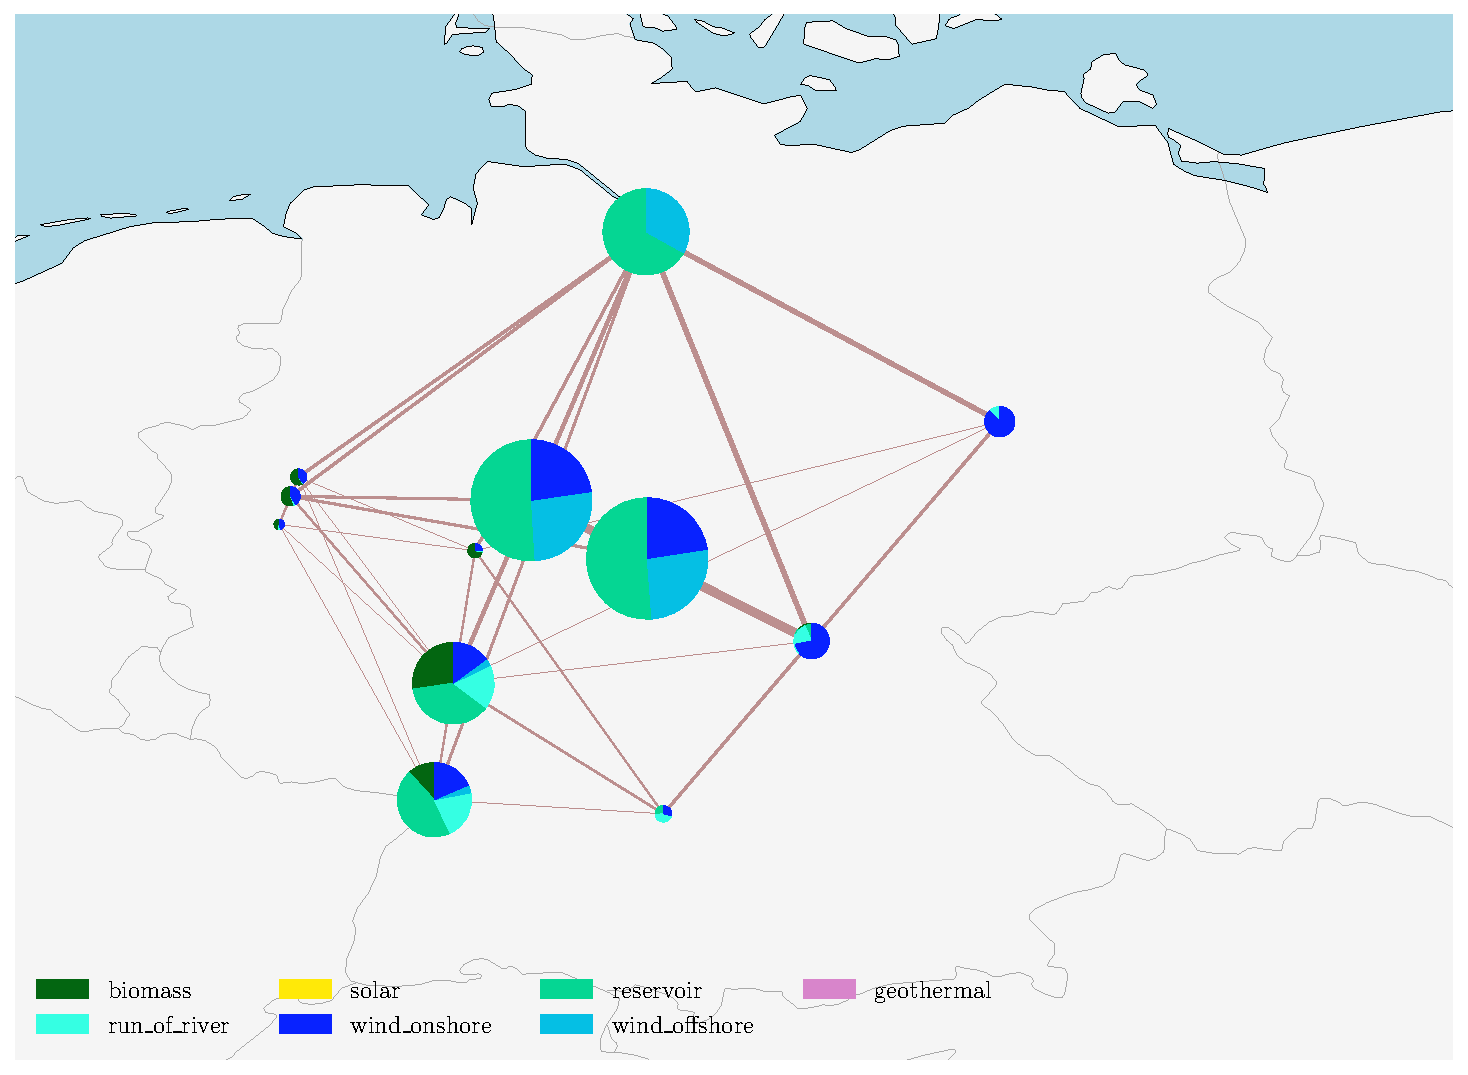
\includegraphics[width=\linewidth]{Figures/eGo100_No7.pdf}
\caption{N=12.}
\label{fig:3d}
\end{subfigure}
    
\caption{Germany network generated with PyPSA for $N$ cluster from eGo100 data.}
\label{fig:GeneralNetworks}
\end{figure}
Lastly, we could compare our hybrid quantum-classical algorithm with the ones provided by the quantum solvers. We think that an specific hyrbrid quantum-classical approach should provide a better solution in term of computational time and optimal value, than the general hybrid solvers from D-Wave. Furthermore, we should be able to determine how much quantum solver are we employing in the problem, which do not happen with solvers such as D-Wave where it is not possible to know how much quantum solver we employed in the hybrid approach. 
%% Chapter 5

\chapter{Conclusions and Outlook} % Main chapter title

\label{Chapter5} % For referencing the chapter elsewhere, use \ref{Chapter5} 

%----------------------------------------------------------------------------------------


%----------------------------------------------------------------------------------------

\section{Conclusions}

\section{Future Work}
\begin{itemize}
    \item PyPSA plots for different number of cluster to show how can we scale the problem + QUARK for reformulating the problem + ji-j? for Hybrid methods.
    \item Quantinium 32 fully connected qubits paper
    \item Network topology (change)
\end{itemize}

In the original protocol a random criterion of selection is assigned to the neighboring function. However, this function can be optimised for a given problem by changing the selection criterion accordingly so that the configuration space is explored in a clever way. For instance, for a large expansion planning the operational cost of a generator -- the annualised cost per $MWh$ of a carrier (wind energy, solar energy, gas, among others) --  is the term that contribute the most to our total cost function. For this reason, we can decide to generate neighboring configuration such that we start by building those generators with less operational cost. This criterion could also considers the number of snapshots and differences of operational cost with respect the investment planning of each generator and decide accordingly to that.
 

%----------------------------------------------------------------------------------------
%	THESIS CONTENT - APPENDICES
%----------------------------------------------------------------------------------------

\appendix % Cue to tell LaTeX that the following "chapters" are Appendices

% Include the appendices of the thesis as separate files from the Appendices folder
% Uncomment the lines as you write the Appendices

% Appendix A

\chapter{Introduction to Quantum Computing} % Main appendix title
This appendix serves as a quick introduction to quantum computing. We explain the basics concepts without going deeply into their physical meaning or historical approach. For a deeper discussion of the topics described herein, we refer the reader to Refs. \cite{W.Bryon1992HilbertFunctions},  \cite{Scherer2019MathematicsComputing} and \cite{Nielsen2010QuantumInformation}.
\label{AppendixA} % For referencing this appendix elsewhere, use \ref{AppendixA}
%%%%%%%%%%%%%%%%%%%%%%%%%%%%%%%%%%%%%%%%%%%%%%%%%%%%%%%%%%%%%%%%%%%%%%%%%%%%%%%%%%%%%%%%%%%%%%%%%%%%%%%%%%
%     A.1 HILBERT SPACE
%%%%%%%%%%%%%%%%%%%%%%%%%%%%%%%%%%%%%%%%%%%%%%%%%%%%%%%%%%%%%%%%%%%%%%%%%%%%%%%%%%%%%%%%%%%%%%%%%%%%%%%%%%
\section{Hilbert space}
We start by defining the vector space where quantum computing takes place, the Hilbert space, $\mathbb{H}$.
\begin{definition}[Hilbert Space]
A Hilbert space is a special type of linear vector space whose elements are complex-valued \textit{square integrable}\footnote{A function $\psi(x)$ is said to be \textit{square integrable} on a given interval $\left[a, b\right]$ if $\int_{a}^{b}\|\psi(x)\|^{2}dx$ exist with a finite value.} functions, $\psi(x)$, of a real variable $x$, defined on the closed interval $\left[a, b\right]$, equipped with a \textit{complete inner product}, $(\cdot,\cdot)$, in $\mathbb{C}$.
\end{definition}
\begin{definition}[Inner Product]
Given two functions of the Hilbert space, $\psi_{1}$ and $\psi_{2}$, the inner product is defined by
\begin{equation}
    \left(\psi_{1}, \psi_{2}\right) \equiv \int^{b}_{a} \psi_{1}^{*}(x)\psi_{2}(x)dx
\end{equation}
\end{definition}
\begin{corollary}
Given the functions \{$\psi_{1}$,$\psi_{2}$,$\psi_{3}$\} $\in \mathbb{H}$ and \{$\alpha, \beta\} \in \mathbb{C}$, the inner product of the associated Hilbert space satisfies:
\begin{itemize}
    \item Closed operation: $(\psi_{1},\psi_{2})\in \mathbb{C}$
    \item Conjugate symmetry: $(\psi_{1},\psi_{2}) = (\psi_{2},\psi_{1})^{*}$
    \item Linear with respect to the second vector: $(\psi_{1},\lambda \cdot \psi_{2} + \beta\cdot\psi_{3}) = \lambda(\psi_{1},\psi_{2}) + \beta(\psi_{1},\psi_{3})$
    \item Anti-linear with respect to the first vector: $(\lambda \cdot \psi_{1} + \beta \cdot \psi_{2}, \psi_{3}) = \lambda^{*}(\psi_{1},\psi_{3}) + \beta^{*} (\psi_{2},\psi_{3})$
    \item Positive definiteness: $(\psi, \psi) = \lVert \psi \rVert^{2} \in \left[0,\infty\right)$\footnote{The quantity $\lVert \psi \rVert^{2}$ is called the norm of $\psi$. If $\lVert \psi \rVert^{2} = 0$ that does not imply $\psi(x) = 0$ for all $x$ in $\left[a,b\right]$. The function can have nonzero values at some points and the integral will remain zero. The integral roughly computes the area in a given interval, so, if there is just a point not null in the interval the area captured by a point is zero, so its contributions to the integral is zero. In our case the quantity $\lVert \psi \rVert^{2}$ represents the probability density of a given state $\psi$, i.e., if we integrate the whole interval of definition $x \in D$, $\int_{D}\lVert \psi \rVert^{2}dx = 1$.} 
\end{itemize}    
\end{corollary}
\begin{definition}[Distance]
    The distance defined by Hilbert space's inner product is given by
    \begin{equation}
      d \equiv \left|\psi_{2} - \psi_{1}\right| = \sqrt{(\psi_{2}-\psi_{1},\psi_{2}-\psi_{1})}  
    \end{equation}
\end{definition}
\begin{definition}[Completeness of a space]
A complete space is one in which any Cauchy sequence -- of that space -- is convergent, i.e., tends towards a value inside the given space.
\end{definition}
We can show why completeness of space is a necessary condition. Suppose that our space is not complete, i.e., some Cauchy sequences are not convergent. Then, the evolution of an initial state\footnote{The formulae for the evolution of n state is explained in later sections.}, $\ket{\psi(0)}$, under a given constant Hamiltonian is not guaranteed\footnote{It is not guaranteed that the Cauchy sequence $\sum_{i = 0}^{n}(-it)^{k} / \left(k!h^{k}\right)\mathcal{H}^{k}$ converges.}
\begin{equation}
    \ket{\psi(t)} = e^{-\frac{i\mathcal{H}}{\hbar}t}\ket{\psi(0)} = \lim_{n \to \infty} \sum_{i = 0}^{n}\frac{(-it)^{k}}{k!h^{k}}\mathcal{H}^{k}\ket{\psi(0)}
\end{equation}
\begin{definition}[Completeness of an orthonormal set of functions]
A set of orthonormal functions $\{\psi_{i}\}$ is complete if any function $\psi(x)$ in Hilbert space can be written as a linear combination of the $\psi_{i}(x)$\footnote{Here we do not ask for point convergence, we weaken the converge criteria to mean convergence. Otherwise, there would not exist a complete set of orthonormal function in the Hilbert space.}:
\begin{equation}
    \lim_{n\to \infty}\| \psi(x) - \sum_{i=1}^{n}c_{i}\psi_{i}(x)\|^{2} = 0
\end{equation}
\end{definition}
\begin{theorem}[Riesz-Fischer]
Assume the functions $\psi_{1}(x),\psi_{2}(x),\ldots$ are elements of Hilbert space. If
\begin{equation}
    \lim_{n,m\to\infty} \lVert \psi_{n} - \psi_{m}\rVert^{2} \equiv \lim_{n,m\to \infty} \int_{a}^{b} \|\psi_{n} - \psi_{m}\|^{2}dx = 0
\end{equation}
then there exist a square (Lebesgue) integrable function $\psi(x)$ to which the sequence $\psi_{n}(x)$ converges such that 
\begin{equation}
    \lim_{n\to \infty} \int_{a}^{b} \|\psi - \psi_{n}\|^{2}dx = 0
\end{equation}
Equivalently, let $\psi_{n}$ be a Cauchy sequence and $\psi$ a value inside the given space. Then, the Cauchy sequence converges to $\psi(x)$ \textit{in the mean}, i.e, we allow the difference $\|\psi(x) - \psi_{n}(x)\|^{2}\neq 0$ at some points $x$, so that the integral $\lim_{n\to \infty} \int_{a}^{b} \|\psi - \psi_{n}\|^{2}dx$ is zero when taking into account the whole interval.
\end{theorem}
\begin{definition}[Orthonormality]
A given set of functions $\{\psi_{i}\}$ is said to be orthonormal if
\begin{equation}
    \left(\psi_{i}, \psi_{j}\right) \equiv \int_{a}^{b} \psi_{i}^{*}(x)\psi_{j}(x) dx = \delta_{ij} 
\end{equation}
\end{definition}
In the present work we work with a particular Hilbert space, a finite Hilbert space. This implies our space is \textit{separable}.
\begin{definition}[Separable]
    A Hilbert space is said to be \textit{separable} if an only if it has a countable orthonormal basis.
\end{definition}
So for a finite Hilbert space -- which is a countable space -- an orthogonal basis is guaranteed.
%%%%%%%%%%%%%%%%%%%%%%%%%%%%%%%%%%%%%%%%%%%%%%%%%%%%%%%%%%%%%%%%%%%%%%%%%%%%%%%%%%%%%%%%%%%%%%%%%%%%%%%%%%
%     A.2 NOTACION
%%%%%%%%%%%%%%%%%%%%%%%%%%%%%%%%%%%%%%%%%%%%%%%%%%%%%%%%%%%%%%%%%%%%%%%%%%%%%%%%%%%%%%%%%%%%%%%%%%%%%%%%%%
\section{Notation}
\begin{definition}[Dirac's Bra-Ket Notation]
The inner product of an n-dimensional Hilbert space defines a linear map from $\mathbb{H}$ to $\mathbb{C}$
\begin{align*}
  \tau: \mathbb{H}\longrightarrow& \mathbb{C}^{n} \\
  \tau(\psi) \longrightarrow& \begin{bmatrix}
           \alpha_{1} \\
           \vdots \\
           \alpha_{n}
         \end{bmatrix}
\end{align*}  
Conversely, 
\begin{align*}
  \bar{\tau}: \mathbb{H}^{*}\longrightarrow& \mathbb{C}^{n} \\
  \bar{\tau}(\psi)\longrightarrow& 
         \begin{bmatrix}
           \alpha_{1}^{*}, \hdots, \alpha_{n}^{*}
         \end{bmatrix}
\end{align*} 
where $\mathbb{H}^{*}$ denotes the dual space. The dual space $\mathbb{H}^{*}$ is also a Hilbert space with the same dimension as $\mathbb{H}$. 
\begin{itemize}
    \item Elements of a Hilbert space, $\mathbb{H}$ are called \textit{ket-vectors} 
\begin{equation}
    \psi \equiv \ket{\psi} =  \begin{bmatrix}
           \alpha_{1} \\
           \vdots \\
           \alpha_{n}
         \end{bmatrix}
\end{equation}
\item Elements of a dual Hilbert space $\mathbb{H}^{*}$ are called \textit{bra-vectors}
\begin{equation}
    \psi^{*} \equiv \bra{\psi} =  \begin{bmatrix}
           \alpha_{1}^{*}, & \hdots &, \alpha_{n}^{*}
         \end{bmatrix}
\end{equation}
\end{itemize}
\end{definition}

Notice that a bra-vector is just the transpose conjugate of a ket-vector. This is a useful way of mapping a ket-vector of a given Hilbert space into its bra-vector on the associated dual Hilbert space.

\begin{corollary}
    In bra-ket notation, a set of vectors $\{\ket{\psi_{j}}\}$ is said to span $\mathbb{H}$ if we can express any vector $\ket{\psi}$ of that space as a linear combination of the vectors in the given set
    \begin{equation}
        \ket{\psi} = \sum_{j}\alpha_{j}\ket{\psi_{j}}
    \end{equation}
    where the coefficients of the combination $\alpha_{j}$ are complex numbers. In particular, if the set of vectors $\{\ket{\psi_{j}}\}$ are linearly independent and the number of vectors in that set is equal to the dimension of our space, then this set of vectors is a basis set of our space and the previous expression is the so-called basis expansion of $\ket{\psi}$.
\end{corollary}
%%%%%%%%%%%%%%%%%%%%%%%%%%%%%%%%%%%%%%%%%%%%%%%%%%%%%%%%%%%%%%%%%%%%%%%%%%%%%%%%%%%%%%%%%%%%%%%%%%%%%%%%%%
%     A.3 Quantum bits
%%%%%%%%%%%%%%%%%%%%%%%%%%%%%%%%%%%%%%%%%%%%%%%%%%%%%%%%%%%%%%%%%%%%%%%%%%%%%%%%%%%%%%%%%%%%%%%%%%%%%%%%%%
\section{Quantum bits}
A \textit{bit} is the smallest unit of information of classical computing. Analogously, a \textit{qubit} is the smallest unit of information for quantum computing. The following section treats bits and qubits as abstract mathematical objects without their physical implementation. In Appx.\,\ref{AppendixC}, we describe some implementations of a physical qubit.\\\\
A classical bit has two possibles states commonly named $\ket{0}$ or $\ket{1}$\footnote{The name of the states of a bit or qubit is not important. It is just a way of labelling those states.}. However, a quantum bit is a linear combination of states -- \textit{superposition} -- $\{\ket{0}, \ket{1}\}$. The general state of a qubit can be conceived as a vector in a two-dimensional complex vector space, with $\alpha, \beta \in \mathbb{C}$
\begin{equation}
    \ket{\psi} = \alpha \ket{0} + \beta \ket{1} = \alpha \begin{bmatrix}
           1 \\
           0 
         \end{bmatrix}
         +
         \beta
         \begin{bmatrix}
           0 \\
           1 
         \end{bmatrix}
\end{equation}
where $\|\alpha\|^{2} + \|\beta\|^{2}$ = 1, i.e, the state of a qubit is normalized.\\
The last expression can be written in term of two parameters,
\begin{equation}
    \ket{\psi} = \cos{\frac{\theta}{2}}\ket{0} + e^{i\phi}\sin{\frac{\theta}{2}}\ket{1}
\end{equation}
that represent the angles of the Bloch Sphere\footnote{A Bloch sphere is a geometric representation of the state of a single qubit where each axis has two orthogonal states, e.g., the Z-axis has the orthogonal states $\{\ket{0},\ket{1}\}$.}.\\
The states $\ket{0}$ and $\ket{1}$ form a computational basis (orthonormal basis) for the $\mathbb{C}^{2}$ vector space. There are infinite single-qubit basis sets for $\mathbb{C}^{2}$, albeit the ones known as \textit{computational basis} are the ones that build the axis of the Bloch Sphere.
\begin{figure}[H]
\centering
    \includegraphics[scale=0.8]{Figures/BlochSphere.pdf}
    \caption{A Bloch Sphere displaying the state $\ket{\psi}$ of a single qubit.}
    \label{fig:bloch_sphere}
\end{figure}
The Pauli matrices represent a rotation\footnote{Pauli matrices are generators of SU(2) group. A complex exponential can be understood as a rotation around a vector $\vec{n}$ where $e^{i\frac{\theta}{2}(\vec{n}\cdot \vec{\sigma})} = \mathbb{I}\cos{\frac{\theta}{2}} + i(\vec{n}\cdot \vec{\sigma})\sin{\frac{\theta}{2}}$.} around a given axis $\{X, Y, Z \}$. The matrix representation is given by,
\begin{align*}
X \equiv \sigma_{x} = \sigma_{1} = 
    \begin{bmatrix}
           0 & 1 \\
           1 & 0 
         \end{bmatrix} \\
Y \equiv \sigma_{y} = \sigma_{2} = 
    \begin{bmatrix}
           0 & -i \\
           i & 0 
         \end{bmatrix} \\ 
Z \equiv \sigma_{z} = \sigma_{3} = 
    \begin{bmatrix}
           1 & 0 \\
           0 & -1 
         \end{bmatrix}
\end{align*}
The eigenvectors of the Pauli matrices are the computational basis vectors,
\begin{align*}
    \Biggl\{\begin{bmatrix}
           1 \\
           0 
         \end{bmatrix}, \begin{bmatrix}
           0 \\
           1 
         \end{bmatrix} \Biggr\}\equiv \{\ket{0}, \ket{1}\} \in Z_{basis} \\
         \Biggl\{\begin{bmatrix}
           \frac{1}{\sqrt{2}} \\
           \frac{1}{\sqrt{2}} 
         \end{bmatrix}, \begin{bmatrix}
           \frac{1}{\sqrt{2}} \\
           -\frac{1}{\sqrt{2}} 
         \end{bmatrix} \Biggr\}\equiv \{\ket{+}, \ket{-}\} \in X_{basis} \\
         \Biggl\{\begin{bmatrix}
           \frac{1}{\sqrt{2}} \\
           \frac{i}{\sqrt{2}} 
         \end{bmatrix}, \begin{bmatrix}
           \frac{1}{\sqrt{2}} \\
           -\frac{i}{\sqrt{2}} 
         \end{bmatrix} \Biggr\}\equiv \{\ket{R}, \ket{L}\} \in Y_{basis}
\end{align*}
In general, we deal with multiple qubits. The basis for an n-qubit system is just the tensor product of n-single-qubit basis.\\
Suppose we have two qubits. Then, the $Z\otimes Z-basis$ is $\{\ket{00},\ket{01},\ket{10},\ket{11}\}$ and the state of a two-qubit system is described by the linear combination,
\begin{equation}
    \ket{\psi} = \alpha_{00}\ket{00} +\alpha_{01}\ket{01} +\alpha_{10}\ket{10} +\alpha_{11}\ket{11}
\end{equation}
where $\|\alpha_{00}\|^{2} + \|\alpha_{01}\|^{2} + \|\alpha_{10}\|^{2} + \|\alpha_{11}\|^{2} = 1$, i.e., the state is normalized.\\
The normalization condition for an n-qubit system can be written as
\begin{equation}
\sum_{x\in \{0,1\}^{n}}\|\alpha_{x}\|^{2} = 1
\end{equation}
Where the expression $x \in \{0,1\}^{n}$ indicates all the possible tensor product combinations of the n-single-qubit states. These combinations form a basis for the n-qubit system.
%%%%%%%%%%%%%%%%%%%%%%%%%%%%%%%%%%%%%%%%%%%%%%%%%%%%%%%%%%%%%%%%%%%%%%%%%%%%%%%%%%%%%%%%%%%%%%%%%%%%%%%%%%
%     A.4 MEASUREMENTS AND OPERATORS
%%%%%%%%%%%%%%%%%%%%%%%%%%%%%%%%%%%%%%%%%%%%%%%%%%%%%%%%%%%%%%%%%%%%%%%%%%%%%%%%%%%%%%%%%%%%%%%%%%%%%%%%%%
\section{Measurements and Operators}
Quantum mechanics makes predictions about microscopic objects taking into account their statistics\footnote{Measurements in an ensemble of equally prepared states gives quantities distributed around a mean value with a given frequency.}. The predictions have implications for the macroscopic world. In classical computing a system is mostly unaltered by tiny interactions such as light or heat. However, in quantum computing this environment noise is quite important as it modify the state of the system. This noise is a doubled-edged sword as it can be used to modify intentionally the state of a quantum system.
\begin{definition}[Operator]
    An operator $\hat{A}$ is a linear map between Hilbert spaces that satisfy,
    \begin{equation}
        \braket{\hat{A}^{\dagger}\psi|\varphi} = \braket{\psi|\hat{A}\varphi} \forall \psi,\varphi \in \mathbb{H}
    \end{equation}
    where $\hat{A}$ admit a matrix representation and "$\dagger$" means transpose conjugate
\end{definition}
\begin{corollary}
    Given an operator $\hat{A}$, on a finite Hilbert space, the operator is said to be Hermitian if
    \begin{equation}
        \hat{A}^{\dagger} = \hat{A}
    \end{equation}
    Hermitian operators play an important role in quantum physics because their eigenvalues are real and represent measurable physical quantities.
\end{corollary}
\begin{definition}[Observable]
    Given the state of a system $\ket{\psi}$, an \textit{observable} -- represented with an operator $\hat{A}$ -- is the physical quantity we can measure associated with the Hermitian operator $\hat{A}$. The possible observables of an operator are its eigenvalues.
\end{definition}
As an example consider the \textit{Hamiltonian} of a system, $\hat{\mathcal{H}}$. For the present work, the Hamiltonian of a system represents the total energy of the system. So, the associated eigenvalues are the eigenenergies of the system.  
\begin{definition}[Unitary Operator]
    An operator U on $\mathbb{H}$ is unitary if
    \begin{equation}
        U^{\dagger}U =\mathbb{I}
    \end{equation}
where $\mathbb{I}$ is the identity operator.
\end{definition}
\begin{definition}[Expectation Value]
    The expectation value, $<\cdot>$, of an observable is the mean value we get after a sequence of measurements of that observable in an ensemble of equally prepared states.
        Mathematically,
    \begin{equation}
        \langle\hat{A}\rangle_{\ket{\psi}} := \braket{\psi |\hat{A}| \psi}
    \end{equation}
\end{definition}

We can measure a classical bit to check if it is in the state 0 or 1. However, when we measure -- in the Z-basis -- a quantum bit we do not get the parameters $\alpha, \beta$ that describe the qubit state. Instead, we get either $\ket{0}$ or $\ket{1}$ with probabilities $\|\alpha\|^{2}$ and $\|\beta\|^{2}$ respectively. The logic of classical computing is Boolean, this means that if the system is not in the state 0 it must be in state 1. In quantum computing, if the system is not in the state 0 it does not have to be in state 1.   

In a measurement, the general state of the qubit collapses to one of the states of the basis we are using to measure. After this measurement the state of our qubit is fixed and successive measurements will give the same state with probability 1, i.e., measurements collapse a qubit into one of the basis states destroying superposition.\\
Quoting Nielsen and Chuang\,\cite{Nielsen2010QuantumInformation},
\begin{displayquote}
\textit{This dichotomy between the unobservable state of a qubit and the observations we can make lies at the heart of quantum computation and quantum information.}
\end{displayquote}
%%%%%%%%%%%%%%%%%%%%%%%%%%%%%%%%%%%%%%%%%%%%%%%%%%%%%%%%%%%%%%%%%%%%%%%%%%%%%%%%%%%%%%%%%%%%%%%%%%%%%%%%%%
%     A.5 SCHRODINGER EQUATION
%%%%%%%%%%%%%%%%%%%%%%%%%%%%%%%%%%%%%%%%%%%%%%%%%%%%%%%%%%%%%%%%%%%%%%%%%%%%%%%%%%%%%%%%%%%%%%%%%%%%%%%%%%
\section{Schrödinger Equation}
One of the paradigms of universal quantum computing is the gate model. This approach substitutes classical logic gates -- such as OR, XOR, AND or NOT -- by its quantum analog. These quantum gates are represented by unitary matrices, so that the inner product is preserved.\\
Equivalently, a quantum gate is represented by a complex exponential of the form\footnote{Where $\hbar$ is the reduced Planck constant.} $\exp\left(i\hat{\mathcal{H}}t / \hbar\right)$ where a given Hamiltonian, $\mathcal{H}$ -- controlled by external fields such as magnetic fields -- leads the evolution of the qubit in such a way that the associated matrix of the complex exponential -- that admit a series expansion -- match the matrix representation of the quantum gate. \\\\
Precisely, the evolution of a quantum system is goberned by the Schrödinger equation which cannot be derived from first principles, i.e., it is an experimental fact. Mathematically, it can be expressed as
\begin{equation}
    \hat{\mathcal{H}}\ket{\psi(t)} = i\hbar \frac{\partial}{\partial t}\ket{\psi(t)}
\end{equation}
where $\hat{\mathcal{H}}$ is the Hamiltonian operator, $\hbar$ is the reduced Planck constant and $\ket{\psi(t)}$ represents the state of a system.\footnote{Remember that in Quantum Physics time does not have an operator so it is not an observable.} and $\ket{\psi(t)}$ represent the state of a system.\\
The Schrödinger equation governs the time evolution of a quantum system. It plays the same role that Newton's equations do in classical mechanics.
%%%%%%%%%%%%%%%%%%%%%%%%%%%%%%%%%%%%%%%%%%%%%%%%%%%%%%%%%%%%%%%%%%%%%%%%%%%%%%%%%%%%%%%%%%%%%%%%%%%%%%%%%%
%     A.6 SPEED-UP ADVANTAGE
%%%%%%%%%%%%%%%%%%%%%%%%%%%%%%%%%%%%%%%%%%%%%%%%%%%%%%%%%%%%%%%%%%%%%%%%%%%%%%%%%%%%%%%%%%%%%%%%%%%%%%%%%%
\section{Speed-up advantage}
We end up this appendix by discussing the main features of quantum behavior that speed-up the algorithms versus its classical approach.\\\\
The main power of quantum computers underlies in three properties,
\begin{itemize}
    \item \textbf{Superposition:} A qubit can be a in a linear combination of states. We can build quantum algorithms that cross out those terms that are not interesting for us and increase the amplitudes of the ones we are interested in.
    \item \textbf{Entanglement:} An entangled state is a state that cannot be written in term of the tensor product of pure states. Entangled states store information exponentially instead of linearly (as classical computing does). As an example, suppose we have the following two-qubit state, called \textit{Bell state}
\begin{equation}
    \ket{\psi} = \frac{1}{\sqrt{2}}\left(\ket{00} + \ket{11}\right)
\end{equation}
If we measure the first qubit in the Z-basis, we can get either the state $\ket{0}$ or $\ket{1}$. We can see that both qubits are entangled in the sense that knowing the state of the first qubit allows us to determine the state of the second qubit. In this case, if the first qubit measurement is $\ket{0}$ we know that the second qubit must be in state $\ket{0}$.\footnote{Einstein termed this effect \emph{spooky action at a distance} in an attempt to ridicule quantum mechanics.}  
    \item \textbf{Parallelism:} A quantum memory register can exist in a superposition of states. If we perform an operation on this quantum register, this operation is applied to all states of that superposition. Notice that we have applied an operation to all the states in that superposition by performing the function just once.
\end{itemize}
Despite the advantage of using quantum computing with respect to classical computing has been proven theorically for some specific problems, see Ref. \cite{Grover19961996Search}, the real world problems are yet far away from being addressed fully by quantum computing\footnote{Nowadays, the hardware is not mature enough for real world industry problems.}. The best we can do nowadays is to solve problems by splitting them into a quantum part that can be done by a quantum computer and a classical part that is solved by using an HPC.
%%%%%%%%%%%%%%%%%%%%%%%%%%%%%%%%%%%%%%%%%%%%%%%%%%%%%%%%%%%%%%%%%%%%%%%%%%%%%%%%%%%%%%%%%%%%%%%%%%%%%%%%%%
%     A.6.1 Grover's Algorithm
%%%%%%%%%%%%%%%%%%%%%%%%%%%%%%%%%%%%%%%%%%%%%%%%%%%%%%%%%%%%%%%%%%%%%%%%%%%%%%%%%%%%%%%%%%%%%%%%%%%%%%%%%%
\subsection{Grover's Algorithm}
In this section we show the advantages of quantum computing by considering a specific example, that of Grover's algorithm.\\
Grover's algorithm is a search algorithm that uses qubits in superposition adjusting their phases to make the computations by quantum parallelism. Given a table with a number of items \textit{N}, we are interested in a particular item $\omega$. The best known classical algorithm can solve the problem in $O(N)$ complexity, which means that in the worst case a classical algorithm has to check each entry of the data-set until finding the item $\omega$ in the last query. Grover's algorithm can solve the problem in $\sim$ $O(\sqrt{N})$ complexity\footnote{This is a lower bound but in some cases the speed up could be better as it happens with the two-qubit system.}, which represent a quadratic speed up compared with the classical approach, i.e., after $\sqrt{N}$ evaluations it is guaranteed to provide the desired state.
\begin{figure}[H]
    \includegraphics[width=\textwidth]{Figures/Grover_Circuit.pdf}
    \caption{Circuit scheme of Grover's algorithm for an n-qubit system.}
    \label{fig:Grover_circuit}
\end{figure}
\subsubsection{Grover's Algorithm steps for a two-qubit system ($N=4$)}
In this section we show what is the state of the system at each step -- after the application of the quantum gates -- and a geometrical representation based on Ref. \cite{Lavor2008Search} and \textbf{REF}.\\
As an example consider the following table,
\begin{table}[H]
\centering
\label{tab:GroverSearch}
\begin{tabular}{ c | c | c | c | c }
  \hline			
  Binary Index & 00 & 01 & 10 & 11 \\
    \hline		
  Item & 0 & 1 & 2 & 3 \\
  \hline  
\end{tabular}
\caption{Grover's search example. Different items described by its binary expansion.}
\end{table}
and suppose we want to find the item 2, where the index -- binary expansion of decimal index starting from zero -- represents the eigenstate of the system we are looking for. Then, if we are interested in finding the item 2, we are looking for the eigenstate $\ket{\omega} = \ket{10}$.\\
\textbf{(0). Initialized single qubit states:} All the qubits are initialized at $\ket{0}$ so the state of the system is given by the tensor product of the qubits,
\begin{equation}
    \ket{\psi_{0}} = \ket{0}\otimes \ket{0} = \ket{00}
\end{equation}
\textbf{(1). Equiprobability:} Apply a Hadamard gate to each qubit so we create a configuration of equiprobable states\footnote{At the beginning we do not have a good guess of where the item can be so each possibility is equally probable.},
\begin{equation}
    \ket{\psi_{1}} = \hat{H}^{\otimes 2}\ket{00} = \frac{1}{\sqrt{N}}\sum_{x \in \{0,1\}^{2}}\ket{x} \equiv \ket{s}
\end{equation}
 One can label the states using decimal notation, $i = 0 ,\ldots, 2^{n} -1$, where $n$ is the number of qubits.\\
For a two-qubit system,
\begin{equation}
   \{\ket{x}\} = \{\ket{00},\ket{01},\ket{10},\ket{11}\} \equiv \{\ket{0},\ket{1},\ket{2},\ket{3}\} = \{\ket{i}\}
\end{equation}
Therefore, we can re-write the state $\ket{s}$ as
\begin{equation}
    \ket{s} = \frac{1}{\sqrt{N}}\ket{\omega} + \frac{1}{\sqrt{N}}\sum_{i \neq \omega} \ket{i}
\end{equation}
Due to the orthonormality of the basis, $\ket{\omega}$ is orthogonal to $\sum_{i \neq \omega} \ket{i}$. So, we can write
\begin{equation}
    \ket{s} = \sin{\theta}\ket{\omega} + \cos{\theta}\ket{s'}
\end{equation}
where
\begin{equation}
    \sin{\theta} = \frac{1}{\sqrt{N}}, \quad\quad  \ket{s'} = \frac{1}{\cos{\theta}}\frac{1}{\sqrt{N}}\sum_{i\neq \omega}\ket{i}
\end{equation}
\begin{figure}[H]
\centering
    \includegraphics[scale=0.55]{Figures/Grover_Step1.pdf}
    \caption{Amplitude distribution of states after applying a Hadamard gate. The vector $\ket{\omega}$ is our desired state and $\ket{s'}$ is a orthogonal vector. In this way we can write $\ket{s} = \sin{\theta}\ket{\omega} + \cos{\theta}\ket{s'}$.}
    \label{fig:Grover_step1}
\end{figure}
\textbf{(2). Reflection about the state $\ket{s'}$:} Apply an operator $\hat{U}_{\omega}$ defined by
\begin{equation}
     \begin{cases}
       \hat{U}_{\omega}\ket{\omega} = -\ket{\omega} \\
       \hat{U}_{\omega}\ket{i} = \ket{i}, &  \forall \ket{i}\neq \ket{\omega} \\
     \end{cases}
\end{equation}
so the operator can be written as,
\begin{equation}
    \hat{U}_{\omega} = \mathbb{I} - 2\ket{\omega}\bra{\omega}
\end{equation}
Applying the operator to the state $\ket{s}$ yields,
\begin{equation}
    \ket{\psi_{2}} = \hat{U}_{\omega}\ket{s} = \ket{s} -\frac{2}{\sqrt{N}}\ket{\omega} \equiv \ket{\bar{s}}
\end{equation}
\begin{figure}[H]
\centering
    \includegraphics[scale=0.55]{Figures/Grover_Step2.pdf}
    \caption{Amplitude distribution of states after applying a $U_{\omega}$. Notice that we have applied a phase to the state we are looking for. Geometrically this means we have applied a reflection about a state orthonormal to $\ket\omega$.}
    \label{fig:Grover_step2}
\end{figure}
\textbf{(3). Reflection about the state $\ket{s}$:} The operator $\hat{U}_{s}$ is defined as,
\begin{equation}
    \hat{U}_{s} \equiv 2\ket{s}\bra{s} - \mathbb{I}
\end{equation}
Applying the operator to the state of our system yields,
\begin{align*}
    \ket{\psi_{3}} = \hat{U}_{s}\left(\ket{s} -\frac{2}{\sqrt{N}}\ket{\omega}\right) = \left(2\ket{s}\bra{s} - \mathbb{I}\right)\left(\ket{s} - \frac{2}{\sqrt{N}}\ket{\omega}\right) = \frac{N - 4}{N}\ket{s} + \frac{2}{\sqrt{N}}\ket{\omega} \\
    = \frac{1}{N\sqrt{N}} \left[\left(N - 4\right)\sum_{x\neq \omega}\ket{x} + \left(3N-4\right)\ket{\omega}\right] \overset{N=4}{=} \frac{1}{8} \left[0 \cdot \sum_{x\neq \omega}\ket{x} + 8\ket{\omega}\right] = \ket{\omega}
\end{align*}
\begin{figure}[H]
\centering
    \includegraphics[scale=0.55]{Figures/Grover_Step3.pdf}
    \caption{Amplitude distribution of states after applying $\hat{U}_{s}$. For the case of two qubits, the amplitudes of non-desired states go to zero so we get the desired state $\ket{\omega}$ with a 100\% of probability in an ideal quantum computer. This does not happen if the number of qubits is increased. In that case the amplitudes of non-desired states are reduced compared with the amplitude of the state we are looking for.}
    \label{fig:Grover_step3}
\end{figure}

We have rotated the original state of our system towards the eigenvector $\ket{\omega}$ that represents the item we are looking for in the data-set. The closer\footnote{Notice that the word "close" in this context is referring to the probability of getting the desired state $\ket{\omega}$ when we make a measurement on the system} we want to be to $\ket{\omega}$ the more times we have to repeat \textbf{(2)} and \textbf{(3)}. The quadratic speed up comes from the fact that Grover's algorithm raises the probability amplitude of the item we are looking for by a factor of $\frac{1}{\sqrt{N}}$ .


%Last Comment


% Appendix B

\chapter{Simulated Annealing} % Main appendix title

This appendix justifies the name of the quantum approach we use in the present work -- \textit{Quantum Anneling} (QA) -- to solve \textit{Quadratic Unconstrained Binary Optimization} (QUBO) problems. In the next sections, we show that the expressions we get in the classical approach known as \textit{Simulated Annealing} (SA), have the same functional form as the ones we get with QA \cite{Kadowaki1998QuantumModel}. To do that we are going to develop the solution for a stochastic problem. For a better understanding about stochastic problems see \cite{Schneider2006StochasticOptimization}. 
\label{AppendixB} % For referencing this appendix elsewhere, use \ref{AppendixB}
%%%%%%%%%%%%%%%%%%%%%%%%%%%%%%%%%%%%%%%%%%%%%%%%%%%%%%%%%%%%%%%%%%%%%%%%%%%%%%%%%%%%%%%%%%%%%%%%%%%%%%%%%%
%     B.1 MASTER EQUATION
%%%%%%%%%%%%%%%%%%%%%%%%%%%%%%%%%%%%%%%%%%%%%%%%%%%%%%%%%%%%%%%%%%%%%%%%%%%%%%%%%%%%%%%%%%%%%%%%%%%%%%%%%%
\section{Master Equation}
A master equation is used to characterize the time-evolution of a given system that switches between states according to a transition rate for a given distribution.
\subsection{Discrete Processes}
Suppose we have a space of states $\Gamma = \{\uparrow \uparrow,\downarrow \uparrow,\uparrow \downarrow,\downarrow \downarrow \} \equiv \{1, 2, 3, 4 \}$ and a discrete stochastic process, e.g. $\{X_{t}, t= 0,1,2,...\} \rightarrow \{1,4,2,3,1,..\}$. Furthermore, assume that the actual setting of our system only depends on the previous one, i.e., the probability of being in state \textit{j} at time \textit{t+1}, $X_{t+1}= j$, given that the current state is \textit{i}, $X_{t} = i$, does not depend on previous configurations.\\
Mathematically,
\begin{equation}
\label{eq: MarkovChain}
    P\left(X_{t+1} = j | X_{t} = i\right) = P\left(X_{t+1}=j | X_{t} = i, X_{t-1} =i_{t-1},...,X_{0} = i_{0}\right)
\end{equation}
The equation \ref{eq: MarkovChain} is known as \textbf{Markov chain} condition and the conditional probabilities are named \textit{transition probabilities}.\\
The normalization condition for probabilities is also fulfilled, i.e., starting from a state  \textit{i} any state \textit{j} -- where \textit{j} can be also the current state -- has a transition probability such that
\begin{equation}
    \sum_{j}P\left(X_{t+1} = j | X_{t} = i\right) = 1, \;\; \forall i
\end{equation}
Graphically, this means that the current state of our systems has to be in a given state of $\Gamma$ at any time.
\begin{figure}[H]
    \centering
    \includegraphics[scale=0.65]{Figures/SA_StateJump.pdf}
    \caption{Stochastic Process for a configuration space $\Gamma$ of four states.}
    \label{fig:SimulatedAnneling_StatesJump}
\end{figure}
\begin{theorem}[Total Probability]
Given an event A in a discrete set of events $\{B_{i}\}$, the probability of occurrence of event A is given by,
\begin{equation}
    P\left(A\right) = \sum_{i}P\left(A|B_{i}\right)P\left(B_{i}\right)
\end{equation}
where $P\left(A|B_{i}\right)$ is the probability of occurrence of event A given that event $B_{i}$ has already happened. 
\end{theorem}
Renaming variables,
\begin{align}
    \label{eq:Renaming1}
    \Pi_{i}(t) \equiv P\left(X_{t} = i\right) \\
    \label{eq:Renaming2}
    p_{i \leftarrow j} := P\left(X_{t+1} = i | X_{t}=j\right)
\end{align}
From equations \ref{eq:Renaming1} and \ref{eq:Renaming2}, we can write,
\begin{align}
        \Pi_{i}(t+1) = p_{i \leftarrow i}\Pi_{i}(t) + \sum_{j \neq i} p_{i \leftarrow j}\Pi_{j}(t) \\ 
        p_{i \leftarrow i} = 1 - \sum_{j\neq i}p_{j \leftarrow i}
\end{align}
Combining the last two equations,
\begin{align}
    \Pi_{i}(t+1) = \left[1 - \sum_{j\neq i}p_{j \leftarrow i}\right]\Pi_{i}(t) + \sum_{j\neq i}p_{i \leftarrow j}\Pi_{j}(t)\\
    \Pi_{i}(t+1) - \Pi_{i}(t) = -\Pi_{i}(t) \sum_{j \neq i}p_{i \leftarrow j} + \sum_{j \neq i} p_{i \leftarrow j}\Pi_{j}(t) \\
    \label{eq: MasterEquationDiscrete}
    d\Pi_{i}(t) := \Pi_{i}(t+1) - \Pi_{i}(t) =  -\Pi_{i}(t) \sum_{j \neq i}p_{i \leftarrow j} + \sum_{j \neq i} p_{i \leftarrow j}\Pi_{j}(t)
\end{align}
we get the master equation of a Markov stochastic discrete process.
\subsection{Continuous Processes}
In case we deal with a continuous process, we need to work with transitions rates defined by,
\begin{equation}
    \mathcal{L}_{i \leftarrow j} = 
    \begin{cases}
    \mathcal{L}_{i \leftarrow j} \;\; i\neq j\\
    -\sum_{k\neq i}\mathcal{L}_{k \leftarrow i} \;\; i = j
    \end{cases}
\end{equation}
so that the master equation can be written as,
\begin{equation}
\label{eq: MasterEquationContinuous}
    \frac{d\Pi_{i}(t)}{dt} = \sum_{j}\mathcal{L}_{i \leftarrow j} \Pi_{j}(t)
\end{equation}
If we know $\Pi_{i}(t_{0})$ we can know the probability at each state. Assume our system has reached the steady state, i.e., $d\Pi_{i}/dt = 0$, which implies,
\begin{equation}
\label{eq: StationaryCondition}
    \Pi_{i}^{\mathrm{eq}} \sum_{j\neq i} \mathcal{L}_{j \leftarrow i} = \sum_{j \neq i}\mathcal{L}_{i \leftarrow j}\Pi_{j}^{\mathrm{eq}} 
\end{equation}
A sufficient but not necessary condition to fulfill \ref{eq: StationaryCondition} is,
\begin{equation}
    \Pi_{i}^{\mathrm{eq}}\mathcal{L}_{j \leftarrow i} = \mathcal{L}_{i \leftarrow j}\Pi_{j}^{\mathrm{eq}} 
\end{equation}
which is known as the \textbf{detailed balanced condition}.\\
The evolution of our system is determined by knowing an initial state and the transition rate expression. Metropolis et al., in connection to statistical mechanics, chose the Boltzmann distribution
\begin{equation}
    \Pi_{i}^{\mathrm{eq}} = \frac{1}{Z}\exp\left(- \frac{\mathcal{H}_{i}}{k_{B}T}\right), \;\;\; Z = \sum_{i}\exp\left(-\frac{\mathcal{H}_{i}}{k_{B}T}\right)
\end{equation}
which implies,
\begin{equation}
    \frac{\mathcal{L}_{j \leftarrow i}}{\mathcal{L}_{i \leftarrow j}} = \exp\left(\frac{\mathcal{H}_{i} - \mathcal{H}_{j}}{k_{B}T}\right)
\end{equation}
The last expression does not define uniquely the transition rate so we need a criterion for that. There are two common criteria:
\begin{itemize}
    \item\textbf{Metropolis criterion:} $\mathcal{L}_{j \leftarrow i} = \min \left[1,\exp\left(\mathcal{H}_{i}-\mathcal{H}_{j}/\left(k_{B}T\right)\right)\right]$. This condition guarantees a transition into states with lower energy without forbidding a transition to higher energy states, where this transition rate depends on the energy difference. 
    \item \textbf{Heat bath criterion:} $\mathcal{L}_{i \leftarrow j} = \frac{\Pi_{j}^{\mathrm{eq}}}{\Pi_{i}^{\mathrm{eq}} + \Pi_{j}^{\mathrm{eq}}} = \left[1 + \exp\left(\frac{\mathcal{H}_{j}- \mathcal{H}_{i}}{k_{B}T}\right)^{-1}\right]$ 
\end{itemize}
 The transition rates do not guarantee the optimal value of our objective function. We must include a time-dependent temperature that guarantees reaching the optimal value when $t \rightarrow \infty$. 
\subsection{Annealing schedules}
The annealing approach considers a temperature that starts from a high value and decreases gradually with time. The dependence of temperature with respect to time $t$ is named annealing schedule. There are many annealing schedules but the most common ones are \footnote{From now on, $k_{B} = 1$.}:
\begin{itemize}
    \item \textbf{Geman-Geman:} This schedule guarantee to reach the absolute minima, see \cite{Geman1984StochasticImages}, in $t \rightarrow \infty$. Mathematically, $T(t) = \frac{a}{b + \log{t}}$
\end{itemize}
Since we do not have infinite time to perform our simulations, we need schedules that are faster despite they do not guarantee convergence to global minimum. 
\begin{itemize}
    \item \textbf{Lineal cooling:} $T(t) = a - bT$ where $a = T_{0}$ -- initial temperature -- and $b \in (0.01,0.2)$.
    \item \textbf{Exponential cooling:} $T(t) = ab^{t}$ where $a = T_{0}$ -- initial temperature -- and $b \in (0.8,0.999)$.
\end{itemize}

%%%%%%%%%%%%%%%%%%%%%%%%%%%%%%%%%%%%%%%%%%%%%%%%%%%%%%%%%%%%%%%%%%%%%%%%%%%%%%%%%%%%%%%%%%%%%%%%%%%%%%%%%%
%     B.2 TSP Example
%%%%%%%%%%%%%%%%%%%%%%%%%%%%%%%%%%%%%%%%%%%%%%%%%%%%%%%%%%%%%%%%%%%%%%%%%%%%%%%%%%%%%%%%%%%%%%%%%%%%%%%%%%
\section{Travel Salesman Problem (TSP) by Simulated Annealing (SA)}
\begin{figure}[H]
\centerline{\includegraphics[width=20cm, height=6cm]{Figures/TSP_SA.pdf}}
    \caption{\textbf{Travel Salesman Problem (TSP) using Simulated Annealing (SA):}\textbf{Left:}, \textbf{Middle:}, \textbf{Right:}}
    \label{fig:TSP_SA}
\end{figure}

% Appendix C

\chapter{Hardware} % Main appendix title
\label{AppendixC} % For referencing this appendix elsewhere, use \ref{AppendixB}
In this Appendix we give an overview of the current quantum hardware without going deeply into details of its implementation. For a better understanding of the implementation of a superconducting qubit -- the ones used by D-Wave -- see Ref.\,\cite{AlvaroDiazComputacionAdiabatica}.
\section{Quantum Technologies}
In classical computing, the \textit{central processing unit} (CPU) is the part of a classical computer that processes the data and performs calculations. The key components of a CPU are called transistors. According to Moore's law, the number of transistors integrated in a micro-controller is doubled every two years. Equivalently, the size of transistors is getting smaller every two years. However, we are approaching the size where quantum effects are starting to appear and have to be taken into account. For this reason, a \textit{quantum processing unit} (QPU) is required. There are different ways of implementing a qubit physically. We summarise some of them in the next table.
\begin{table}[H]
\centering
\begin{tabular}{ |c|c|c|c|c|  }
 \hline
 \multicolumn{2}{|c|}{\textbf{Qubit implementation technologies}} \\
 \hline
 \textbf{Name} & \textbf{Companies}  \\
 \hline
Superconducting qubits         & IBM, D-Wave, Rigetti, IQM \\
 \hline
Trapped ions         & IONQ, Quantinuum, Oxford Ionics, EleQtron \\
 \hline
Photons     & Xanadu, Orca Computing, PsiQuantum, Quandela \\
 \hline
Anyons      & Microsoft \\
 \hline
\end{tabular}
\caption{List of current ways of implementing a qubit and the companies that are are developing them..}
\label{tab:QubitTechnologies}
\end{table}
Concretely, we are interested in the implementation of D-Wave's superconducting qubits. However, a detailed explanation would be lengthy and we will only provide a simple overview of the historical evolution of D-Wave's annealers in terms of number of qubits and connectivity. More details can be found in Ref.\,\cite{AlvaroDiazComputacionAdiabatica}. \\\\
Quoting DiVicenzo\,\cite{Divincenzo2000TheComputation}, the following criteria have to be fulfilled for the realisation of a quantum computer:
\begin{displayquote}
\begin{itemize}
    \item \textit{A scalable physical system with well characterized qubits.}
    \item \textit{The ability to initialize the state of the qubits to a simple fiducial state, such as} $\ket{000...}$.
    \item \textit{Long relevant decoherence times, much longer than the gate operation time.}
    \item \textit{A "universal" set of quantum gates.}
    \item \textit{A qubit-specific measurement capability.}
\end{itemize}
\end{displayquote}
\section{Quantum Annealers: An Overview} 
Quantum annealers are single-purpose quantum computers that solve Ising/QUBO problems. D-Wave started using using d-wave superconductors -- from where D-Wave takes its name -- but in 2011 D-Wave's researchers demonstrated a way of implementing synthetic qubits\,\cite{Johnson2011QuantumSpins}, i.e., qubits that interact between each other and whose behaviour is that of the Ising model. Here we show a list of D-Wave's quantum annealers.
\begin{table}[H]
\centering
\begin{tabular}{ |c|c|c|c|c|  }
 \hline
 \multicolumn{5}{|c|}{\textbf{D-Wave quantum annealers}} \\
 \hline
 \textbf{Name} & \textbf{Release} & \textbf{No. of physical qubits} & \textbf{Architecture} & \textbf{Connectivity}\\
 \hline
 D-Wave One         & 2011 & 128      & Chimera & 6\\
  \hline
 D-Wave Two         & 2013 & 512      & Chimera & 6\\
  \hline
 D-Wave 2$\chi$     & 2015 & 1152     & Chimera & 6\\
  \hline
 D-Wave 2000Q       & 2017 & 2048     & Chimera & 6\\
  \hline
 D-Wave Advantage   & 2020 & 5640     & Pegasus & 15\\
  \hline
 D-Wave Advantage 2 & $\sim$2024 & 7440 & Zephyr  & 20\\
 \hline
\end{tabular}
\caption{Evolution of D-Wave quantum annealers.}
\label{tab:DwaveAnnealers}
\end{table}
Notice that the number of qubits is increasing every few years, almost duplicating its number. However, the number of qubits is not the only factor to care about but the connectivity of those qubits. The connectivity is given by the architecture, it represents the number of different qubits to which a given qubit is connected. Once a QUBO problem is formulated, D-Wave maps it into a Ising problem and it tries to embed the problem into the hardware. If a possible embedding is found, then the problem can be executed in a quantum annealer. This embedding depends on the number of variables our system has and on the entangled qubits required. In order to be able to solve a problem with the same number of binary variables as the number of physical qubits of a quantum annealer, the quantum annealer must have fully-connected qubits. We are yet far away from this fully-connected architecture, even though the connectivity between qubits is increasing every few years as Table\,\ref{tab:DwaveAnnealers} shows.
% Appendix D

\chapter{Python Scripts} % Main appendix title

This appendix contains all the scripts used in the thesis. These scripts can be found at my GitHub repository LopezBanos.
\label{AppendixD} % For referencing this appendix elsewhere, use \ref{AppendixB}
%%%%%%%%%%%%%%%%%%%%%%%%%%%%%%%%%%%%%%%%%%%%%%%%%%%%%%%%%%%%%%%%%%%%%%%%%%%%%%%%%%%%%%%%%%%%%%%%%%%%%%%%%%
%     D.1 TSP Problem
%%%%%%%%%%%%%%%%%%%%%%%%%%%%%%%%%%%%%%%%%%%%%%%%%%%%%%%%%%%%%%%%%%%%%%%%%%%%%%%%%%%%%%%%%%%%%%%%%%%%%%%%%%
\section{Two Heirs Problem}
%////////////////////
\begin{algorithm}
\caption{Two Heirs Problem}\label{alg:twoheirs}
\begin{algorithmic}
\Require $n \geq 0$
\Ensure $y = x^n$
\State $y \gets 1$
\State $X \gets x$
\State $N \gets n$
\While{$N \neq 0$}
\If{$N$ is even}
    \State $X \gets X \times X$
    \State $N \gets \frac{N}{2}$  \Comment{This is a comment}
\ElsIf{$N$ is odd}
    \State $y \gets y \times X$
    \State $N \gets N - 1$
\EndIf
\EndWhile
\end{algorithmic}
\end{algorithm}
%////////////////////
\inputminted[linenos]{python}{Scripts/Two_Heirs.py}
\section{Traveling Salesman Problem}
%////////////////////
\begin{algorithm}
\caption{Travelling Salesman Problem}\label{alg:tsp}
\begin{algorithmic}
\Require $n \geq 0$
\Ensure $y = x^n$
\State $y \gets 1$
\State $X \gets x$
\State $N \gets n$
\While{$N \neq 0$}
\If{$N$ is even}
    \State $X \gets X \times X$
    \State $N \gets \frac{N}{2}$  \Comment{This is a comment}
\ElsIf{$N$ is odd}
    \State $y \gets y \times X$
    \State $N \gets N - 1$
\EndIf
\EndWhile
\end{algorithmic}
\end{algorithm}
%////////////////////
\inputminted[linenos]{python}{Scripts/tsp_simulated_annealing.py}
\section{Transmission expansion problem: A three node example}
%////////////////////
\begin{algorithm}
\caption{Transmission Expansion Planning Problem}\label{alg:tep}
\begin{algorithmic}
\Require $n \geq 0$
\Ensure $y = x^n$
\State $y \gets 1$
\State $X \gets x$
\State $N \gets n$
\While{$N \neq 0$}
\If{$N$ is even}
    \State $X \gets X \times X$
    \State $N \gets \frac{N}{2}$  \Comment{This is a comment}
\ElsIf{$N$ is odd}
    \State $y \gets y \times X$
    \State $N \gets N - 1$
\EndIf
\EndWhile
\end{algorithmic}
\end{algorithm}
%////////////////////
\section{Quantum Benders Decomposition algorithm for TEP problems}
%\include{Appendices/AppendixC}

%----------------------------------------------------------------------------------------
%	BIBLIOGRAPHY
%----------------------------------------------------------------------------------------

\printbibliography[heading=bibintoc]

%----------------------------------------------------------------------------------------

\end{document}  
